% sample article for KAIS
% last modified by alison woollatt, 18 jan 00
% minor changes by xindong wu, 2 march 01

\documentclass{kais}
%
\usepackage{wrapfig,epsf,graphicx,mathtools,multirow}
\usepackage[dcucite]{harvard}

\newtheorem{defi}{Definition}[section]
\newtheorem{property}{Property}[section]
\newtheorem{algorithm}{Algorithm}[section]

\newcommand\changenum{%
  \renewcommand\labelenumi{\theenumi}%
  \renewcommand{\theenumi}{(\arabic{enumi})}%
}

\newcommand\changepnum{%
  \renewcommand\labelenumi{\theenumi}%
  \renewcommand{\theenumi}{($P_\arabic{enumi}$)}%
}

%\bibliographystyle{agsm}

\received{xxx}
\revised{xxx}
\accepted{xxx}

\pubyear{2000}
\pagerange{\pageref{firstpage}--\pageref{lastpage}}
\volume{xxx}

\begin{document}
\label{firstpage}

\title{Variability-based improvement of m-learning applications development}

\author[FalvoJr et al]{V.~FalvoJr$^1$, A.~Marcolino$^1$, N.~Duarte~Filho$^1$,E.~OliveiraJr$^2$ and
E.~Barbosa$^1$\\ $^1$University of S\~ao Paulo (USP), S\~ao Paulo, Brazil;\\$^2$State University of Maring\'a (UEM), Paran\'a, Brazil}
 
\maketitle

\begin{abstract}
Software Product Lines (SPL) aim at improving the product quality and time-to-market of the development methodology of singular software. The central concept of such a reuse approach is variability, which provides diversity of software products in a specific domain. In the educational domain, the popularity of mobile devices has contributed to the increasing demand for mobile learning (m-learning) applications. This paper discusses how variability can improve the development of m-learning applications by adoption of the SMarty, a concise variability management approach. An SPL for m-learning applications has been proposed and experimentally evaluated in industry and provided evidences that well-defined variabilities can speed up time-to-market of m-learning products with a reduced number of faults.
\end{abstract}

\begin{keywords}
mobile learning applications; software product lines; variability management; experimental evaluation
\end{keywords}

\section{Introduction}

Constant changes in software reuse approaches have lead to the concept of Software Product Lines (SPL), which represents a shift in focus from the singular software development paradigm. Companies that had developed project-by-project software have now focused on the creation and maintenance of SPL and their variabilities. Therefore, models that represent variabilities are specified as part of the core assets of an SPL and their correct identification, specification and representation provide several development benefits \cite{chen11,capilla13}.

The variabilities management that enable diversification in the portfolio of products in a given domain requires the adoption of a well-defined systematic approach. Some of these approaches can be used in Domain Engineering (DE) and Application Engineering (AE) to support the selection and delimitation of the variant artifacts from different products \cite{bockle05,vanderlinden07}.

For an SPL to be successful, its domain must be carefully defined. If the domain is too large and product members vary widely, the core assets will be strained beyond their ability to accommodate the variation, economies of the production will be lost, and the product line will collapse into an old-style, one-at-a-time product development effort. On the other hand, if the domain is too small, the core assets might not be built in a generic enough fashion to accommodate a future growth and the product line will stagnate, i.e., economies of the domain will never be achieved and the full potential return of investment (ROI) will never materialize \cite{bockle05,vanderlinden07}.

From a different, but related perspective, the rapid growth of information and communication technologies has favored the emergence of innovative ways for facing the shortcomings of traditional education \cite{west12}. Mobile learning (m-learning) for instance, has provided a strong interaction between learners and instructors, enabling them to actively participate in the knowledge construction process anytime and anywhere \cite{kukulska05}. 

M-learning has grown in terms of importance and visibility, mainly because of significant results regarding flexibility and propagation of education \cite{kinshuk03,wexler08}. Such aspects have made m-learning a promising tool for education. In 2011, the first ``UNESCO Mobile Learning Week'' suggested m-learning as an alternative to the ``teacher crisis'', an expression justified by global need for 8.2 million new teachers for the achievement of the UN Millennium Development Goal of providing universal primary education by 2015 \cite{west12}.

Due to the diversity of platforms, technologies and pedagogical methods considered for the development of m-learning applications, a wide range of specificities can be streamlined and addressed from a reuse perspective. However, few studies have focused on development issues through a strategy of systematic reuse, such as SPL, for mobile middleware, hence the m-learning domain \cite{bezerra09}.

Motivated by this scenario, we have worked on the establishment of M-SPLear\allowbreak ning, an SPL to the m-learning domain \cite{falvojr14a,falvojr14b}. M-SPLear\allowbreak ning has been developed based on a concise UML-based variability management approach, named SMarty, which provides mechanisms to facilitate the identification and representation of variabilities \cite{oliveirajr10}.

This paper discusses how variability improves the development of m-learning applications by SMarty. We experimentally evaluated M-SPLear\allowbreak ning regarding singular software development, particularly comparing time-to-market and quality of the software products implemented to the use of both (SPL and singular) approaches. The results showed a significant reduction in the time-to-market and improvement in the quality in terms of faults, when considering the software products developed from the M-SPLear\allowbreak ning core assets with the support of variabilities.

The paper is organised as follows: Section \ref{section2} summarizes the background; Section \ref{section3} describes M-SPLear\allowbreak ning; Section \ref{section4} addresses the experimental evaluation; Section \ref{section5} discusses the lessons learned from the development and application of M-SPLear\allowbreak ning; Section \ref{section6} reviews the related works; finally, Section \ref{section7} provides the conclusions and perspectives for future work.


\section{Background}\label{section2}

This section provides a brief overview of essential concepts related to (i) SPL and variabilities, (ii) the SMarty approach for variability management and (iii) m-learning.

\subsection{SPL and Variabilities}

SPL enable the creation of software-intensive systems that share and manage a set of features for satisfying the specific needs of a particular domain. Commonalities are shared by all derived products, while variabilities represent the scope of customization supported by them \cite{bockle05,vanderlinden07}.

Variability is one of the most important issues in the design of an SPL, as it reflects the way family members of an SPL differ from each other. The precise and explicit representation and management of variabilities enable a consistent generation of specific products in an SPL \cite{chen11,capilla13}. 

Variabilities can be initially identified and represented by means of features, relevant and visible characteristics to stakeholders of a particular domain \cite{bosch01}. Features are usually represented by a feature model, i.e., a hierarchical structure that captures the structural relationships among the features of a specific domain \cite{bockle05,vanderlinden07}. Common features for the SPL products are considered mandatory, while variable features can be optional or alternative.

% 29/12/2015 01:12 %

The concept of SPL is suitable for domains in which products that share common features and a well-defined set of variabilities are demanded. For instance, in the education domain, instructors, tutors and apprentices can use ubiquitous computing to contribute and access the learning materials anytime and anywhere \cite{kukulska05}. This characteristic is achieved due to variabilities, such as interactivity and multimedia resources \cite{falvojr14a,falvojr14b}, which provide a high degree of communication and cooperation among users.

At its essence, the conception of an SPL involves core asset and product development, both under technical and organizational management perspectives. A core asset can be developed through the extraction of artifacts from software products or from scratch. In general, the products and core assets are built according to their domain needs. Such SPL conception phases are classified into three essential activities, namely (i) Core Asset Development or DE, (ii) Product Development or AE and (iii) Management \cite{bockle05,vanderlinden07}.

\subsection{SMarty Approach}

% 29/12/2015 18:50 %

The proper management of variabilities has great relevance to ensure that all the benefits of SPL are obtained. Therefore different approaches related to the management of variabilities have been proposed by the research community, such as SMarty.  \cite{chen11,capilla13}.  

\textbf{S}tereotype-based \textbf{M}anagement of V\textbf{ar}iabili\textbf{ty} (SMarty)~\cite{oliveirajr10} is a variability management approach composed of a UML 2.4 profile (SMartyProfile) and supported by a systematic process (SMartyProcess), related to the main SPL activities. SMartyProcess defines a set of guidelines that supports the application of stereotypes and tagged-values. The guidelines ensure the identification and representation of variabilities and enabled the evolution of SPL, whereas the process incrementally and iteratively guarantees the identification of new variabilities and evolution of the SPL core assets.

Another benefit from the use of SMarty is visibility regarding the relationship among the feature model and variabilities in the UML diagrams. The variabilities composed of variation points are fully represented. Therefore, there are no additional documents for the development of SPL \cite{oliveirajr10}.

The UML models supported by SMarty (use case, class, sequence, component and activity) represent the static and dynamic aspects of software products. The SMarty effectiveness in identifying and representing variabilities in the UML models has been experimentally evaluated \cite{marcolino13,marcolino14a,marcolino14b,bera15}. The results provided initial evidence of the SMarty effectiveness. In addition, they lead to the empirically evolution of SMarty in general.

\subsection{Mobile Learning}

The rapid growth of information and communication technologies has favored the emergence of new methods for teaching and learning and innovative ways for facing the shortcomings of traditional education \cite{west12}. 

M-learning is characterized by its ability to provide a strong interaction between learners and instructors, who not only access a virtual learning environment, but also contribute to and actively participate in the knowledge construction process through mobile devices anytime and anywhere \cite{kukulska05}. Such a interaction through mobile devices provides other benefits than accessibility, convenience and communication.

However, m-learning is still considered an incipient concept, as it has limitations that hamper its effective development and adoption. For instance, even with the increasing demand for m-learning applications, few studies have addressed development issues through a strategy of systematic reuse, such as SPL, in the mobile learning setting.  

Based on the concepts and ideas summarized in this section, we have worked on the establishment of an SPL for the m-learning domain, named M-SPLear\allowbreak ning. Your main characteristics and experimental evaluation are discussed next.


\section{M-SPLearning}\label{section3}

%Com o objetivo de apresentar como o gerenciamento da variabilidades pode melhorar o desenvolvimento de aplicações de m-learning, os autores definiram uma LPS, denominada M-SPLearning. Buscando explorar as variabilidades desse domínio para acelerar o time to market e reduzir o numero de falhas nos produtos. Nesta seção, as atividades conduzidas para a concepção da M-SPLearning são detalhadas a fim de expor suas principais peculiaridades e referências.
Aiming at presenting how the management of variabilities can improve the development of m-learning applications, we have established M-SPLearning \cite{falvojr14a,falvojr14b}. The idea is to investigate how the variabilities of this domain can accelerate time-to-market and reduce product faults. In this section, the activities conducted in design of the M-SPLearning are detailed \cite{oliveirajr10,filho13,krueger02,kang90}.

\subsection{Domain Engineering}\label{section31}

%Durante a atividade de Engenharia Domínio as similaridades e variabilidades devem ser eliciadas para o desenvolvimento de LPS, a fim de estabelecer uma plataforma reutilizável sistemática. O resultado desta atividade é um conjunto de ativos com os quais a LPS deve ser implementada, caracterizando, assim, sua família de produtos. Em geral, as actividades que caracterizam a Engenharia de Domínio pode ser consideradas as mais críticas durante a concepção de uma LPS, dado que delimitar um domínio de estudo não é uma tarefa trivial.
During the DE activity, similarities and variabilities must be specified for the development of the SPL and establishment of a systematic reusable platform. The result is a set of assets from which the SPL should be implemented, which characterizes its product family \cite{bockle05,vanderlinden07}. In general, the activities that characterize the DE can be considered the most critical in the conception of an SPL, since the delimitation of a domain of study is not a trivial task.

%Analisando o extenso domínio das aplicações móveis percebe-se que seus produtos podem ser implementadas usando diferentes plataformas de desenvolvimento, como por exemplo, Android, iOS ou Windows Phone. Com isto, o domínio de m-learning também inclui sistemas operacionais diferentes. Assim, para definir um domínio aceitável em termos de escopo, selecionamos um único sistema operacional. Nossa escolha pelo Android se baseou na quantidade de dispositivos que cada sistema operacional controla, visto que esse SO detém cerca de 80% do mercado de smartphones do mundo, equivalente a 793,6 milhões de dispositivos.
Mobile applications can be implemented through different development platforms, including Android, iOS and Windows Phone. Furthermore, the m-learning domain also includes different operating systems. We selected a single operating system (Android) for the definitions of an acceptable domain in terms of scope, based on the number of devices each operating system control. Such an OS owns approximately 80\% of the world's smartphones market, which is equivalent to 793.6 million devices. \cite{llamas14}.

%Com um domínio factível definido, um catálogo de requisitos para ambientes m-learning foi adaptado respeitando o modelo de qualidade ISO/IEC 25010, gerando, assim, um catálogo de requisitos estendido e, em seguida, o modelo de features para a M-SPLearning. Tal catálogo busca refletir, em alto nível, a experiência adquirida pelos desenvolvedores e pesquisadores nesta nova modalidade de aprendizagem. Além disso, o catálogo é genérico e abrangente, beneficiando sua adoção para fins diferentes do domínio de m-learning.
After feasible domain had been defined, a requirements catalog for m-learning applications based on a related work \cite{filho13} and ISO/IEC 25010 quality model was proposed. It aims at reflecting, in a high level basis, the experience gained from developers and researchers of m-learning. Furthermore, it is generic and comprehensive and its adoption benefits different purposes in the m-learning domain. 

%Para o gerenciamento das variabilidades em questão a M-SPLearning foi desenvolvida com base na abordagem SMarty. Entre as razões para a nossa escolha, destacam-se: (i) a facilidade cognitiva fornecida pela SMarty, apoiada por várias ferramentas de modelagem; (ii) a sua conformidade com UML, facilitando o desenvolvimento e validação da SPLs; e (iii) a existência de evidências experimentais no que diz respeito à sua utilização.
For the management of such variabilities, the development of M-SPLearning was based on the SMarty approach~\cite{oliveirajr10}, because of (i) the cognitive ease provided by SMarty, supported by several modeling tools; (ii) its compliance with UML, which facilitates the development and validation of SPLs; and (iii) the existence of experimental evidence of its use~\cite{marcolino13,marcolino14a,marcolino14b,bera15}. 

%Em termos práticos, as atividades para a implementação de uma LPS não são triviais e exigem tempo e esforço consideráveis, o que compromete a sua aceitação na indústria. Com o objetivo de reduzir as barreiras de adoção desse conceito foram consideradas três estratégias: proativo, reativo e extractivo.
In practical terms, the activities for the SPL implementation are not trivial and require considerable time and effort, which undermines its acceptance in industry. Aiming to define an appropriate adoption strategy to the concept of SPL, the proactive, reactive and extractive models can be considered \cite{krueger02}.
%Tais modelos foram analisados considerando o contexto deste trabalho, assim a abordagem proativa foi escolhida. Essa estratégia é plenamente aplicável ao contexto da M-SPLearning, uma vez que é apropriada quando os requisitos para o conjunto de produtos a serem desenvolvidos são estáveis e podem ser previamente definidos, condição fornecida pelo catálogo de requisitos relacionado à LPS.
Each model was analyzed considering the context of this work, and the proactive approach was chosen. This strategy is fully applicable to the context of M-SPLearning, since it is the most appropriate when the requirements for the set of products to be developed are stable and can be previously defined. This condition was satisfied by the proposed requirements catalog.

\subsubsection{Domain Analysis}\label{domainAnalysis}

%De acordo com o modelo de adoção proativo proposto por \citet{krueger2001}, primeiramente é realizada a Análise de Domínio e escopo, com o propósito de identificar a variação dos produtos apoiados pela LPS. Para isso, o catálogo de requisitos proposto por \citet{filho2013} foi confrontado com o modelo de qualidade ISO/IEC 25010 \cite{iso2011}, com o objetivo de identificar requisitos de qualidade ausentes ou desconexos em termos negociais e hierárquicos.
In relation to the proactive model, the domain and scope analysis should be summarily performed, to that the variation of the products supported by an SPL can be explored \cite{krueger02}. The requirements catalog \cite{filho13} was analysed with respect to quality model ISO/IEC 25010, for the identification of missing or disconnected quality requirements.
%A partir dessa análise alguns requisitos foram reagrupados, renomeados e, em menor proporção, adicionados e removidos do catálogo de requisitos. Essas modificações consideraram o escopo e domínio definidos para a M-SPLearning, gerando assim uma derivação do catálogo original, ilustrado na Figura \ref{fig:msplCatalogo}.
Some requirements have been regrouped, renamed and, in few cases, added to and removed from the catalog. The final requirements catalog is illustrated in Figure \ref{figureMSPLCatalog}.

\begin{figure}
    \centering
    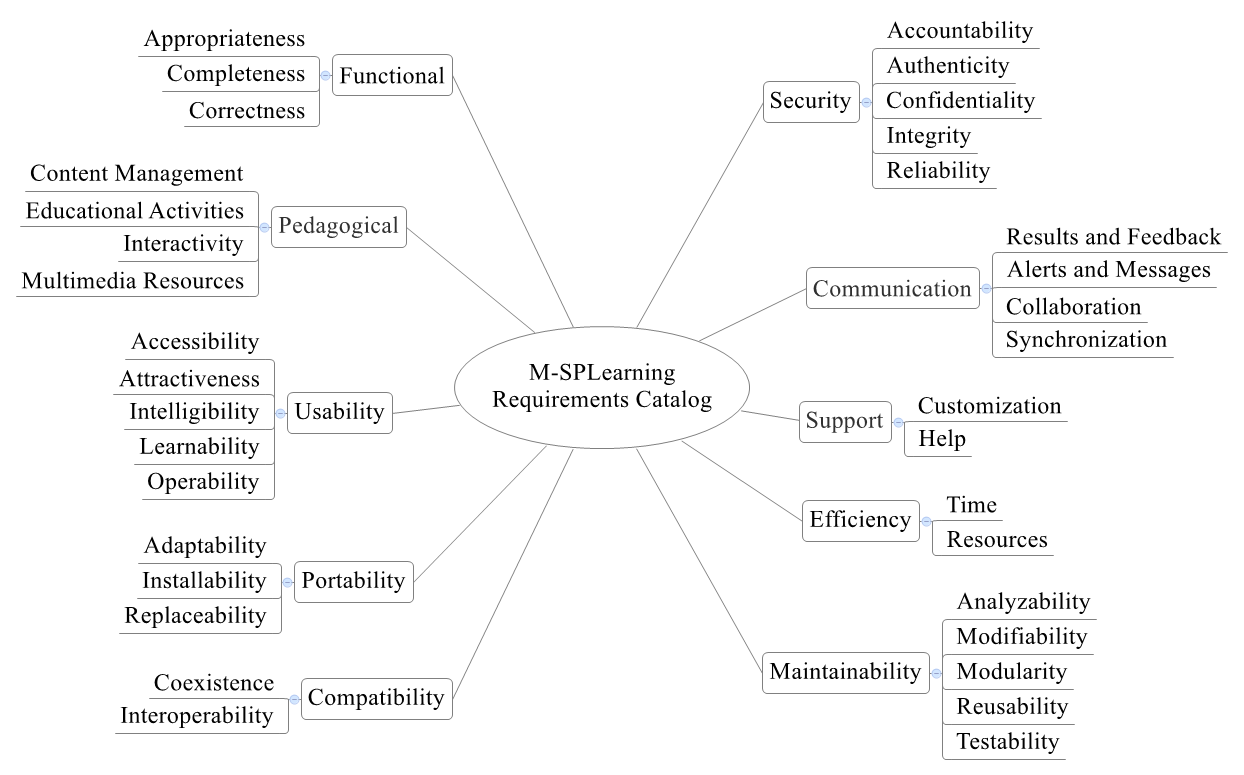
\includegraphics[scale=0.37]{figures/section3/MSPLCatalog}
    \caption{M-SPLearning Requirements Catalog \cite{falvojr14b}.}
    \label{figureMSPLCatalog}
\end{figure}

%Com base no catálogo de referencia, observou-se que a maioria dos requisitos originalmente propostos eram equivalentes, direta ou indiretamente, às características e subcaracterísticas da norma ISO/IEC 25010. Com isso, acredita-se que a derivação do catálogo forneceu os requisitos educacionais móveis necessários para a concepção da LPS deste trabalho.
According the catalog, most requirements originally proposed were directly or indirectly equivalent to the characteristics and subcharacteristics of ISO/IEC 25010. %Thus, it is believed that the performed  derivation provided us the educational requirements necessary for the M-SPLearning.
%Em termos estruturais, o catálogo resultante apresentou 10 requisitos primários e 35 secundários. Por exemplo, o elemento Support apresenta características comuns como a internacionalização de mensagens (provida pelo requisito Customization) e ajuda em dúvidas frequentes (Help).
In structural terms, the resulting catalog has 10 primary and 35 secondary requirements. For example, the \textit{Support} element has common features, such as internationalization of messages (provided by \textit{Customization} requirement) and frequently asked questions (\textit{Help}).

%Apesar de possuir requisitos genéricos e aplicáveis a outros domínios, o catálogo proposto também possui características específicas para aplicações m-learning. Por exemplo, a maior parte dos requisitos derivados a partir de Pedagogical e Communication representam necessidades essenciais ao domínio educacional móvel.
Despite it generic requirements, the catalog also has specific features for m-learning applications. For instance, most requirements derived from \textit{Pedagogical} and \textit{Communication} represent essential requirements to the mobile educational domain.

%Em termos pedagógicos, o gerenciamento de conteúdos educativos é fundamental para o desenvolvimento das atividades educacionais. Além disso, a presença de recursos multimédia pode proporcionar acesso a informação de uma forma mais atrativa. Tais peculiaridades sintetizam os requisitos classificados pelo item Pedagogical.
In pedagogical terms, the management of educational content is essential for the development of educational activities. Furthermore, multimedia resources can provide access to information in a more attractive way. Such peculiarities summarize the requirements classified by the \textit{Pedagogical} item.

%Por sua vez, os requisitos provenientes de Comunucation representam funcionalidades relacionadas à troca de mensagens, alertas e o compartilhamento de resultados ou feedbacks, tornando o aprendizado, mais colaborativo e dinâmico. Outra característica importante é a sincronização dos dados de uma aplicação m-learning, pois os usuários podem possuir e utilizar mais de um dispositivo móvel ou plataforma. 
The requirements from \textit{Communication} represent features related to the exchange of messages, alerts and sharing results or feedback, which make the learning process more collaborative and dynamic. Another important feature is the synchronization of data from a mobile learning application, since users can have more than one mobile device or platform.

%A fim de avaliar o catálogo de requisitos proposto para a M-SPLearning uma validação adicional actividade foi conduzida. Neste sentido, um formulário on-line foi preparado a fim de verificar informalmente as principais questões técnicas relacionadas ao catálogo. O formulário foi disponibilizado em uma estrutura de checklist, com o objetivo de mensurar a opinião de especialistas na área de engenharia de software.
An additional validation activity was conducted for evaluation of the requirements catalog proposed for the M-SPLearning. An online form was prepared for informally checking the main technical issues related to the catalog. It was structured as a checklist, with 12 multiple choice questions so that it could measure the specialists opinions in software engineering area.

%O documento contou com 12 questões de múltipla escolha, onde as duas primeiras eram relacionadas à experiência dos participantes nos conceitos de LPS e m-learning. Nesse caso, as opções possíveis foram: Proficiente, Intermediário e Novato. As dez  questões restantes referiam-se ao catálogo de requisitos da M-SPLearning, por exemplo: O catálogo compreende requisitos adequados ao domínio?. Para essas perguntas as opções: Adequado, Regular e Insatisfatório foram aplicadas.
The first two questions were related to the background of the participants on SPL and m-learning concepts and the options were ``Expert", ``Intermediate" and ``Novice". The ten remaining questions were related to the M-SPLearning requirements catalog, such as \textit{``Does the catalog comprise appropriate requirements to the domain?"}. The options were ``Adequate", ``Regular" and ``Unsatisfactory".

%Os resultados coletados mostraram que, na visão dos participantes, o catálogo de requisitos está adequado ou regular a todos os itens avaliados. Além disso, nenhuma das questões relacionadas ao catálogo de requisitos da M-SPLearning foi respondida como insatisfatória. A Tabela \ref{tableMSPLChecklist} sintetiza as avaliações médias obtidas a partir dos 11 formulários de ckecklist submetidos.
The questionnaire was answered by 11 participants and the results showed the requirements catalog was ``Adequate", with a mean of 60.90\%, and was ``Regular", with a mean of 39.10\%, for all items evaluated. Furthermore, none of the questions related to the M-SPLearning was answered as ``Unsatisfactory". 

%Table \ref{tableMSPLChecklist} summarizes the average ratings obtained.
%
%\begin{table}
%    \caption{M-SPLearning Requirements Catalog Checklist Summary.}
%    \centering
%    \scriptsize
%    \begin{tabular}{cc}
%        \toprule
%        \textbf{Option} & \textbf{Average Percentage Obtained} \\
%        \midrule
%        Adequate       & 60.90\% \\
%        Regular        & 39.10\% \\
%        Unsatisfactory & 0.00\% \\
%        \bottomrule
%    \end{tabular}
%    \label{tableMSPLChecklist}
%\end{table}

Although preliminary, the informal validation performed was important for the evaluation of set of requirements elicited for M-SPLearning.

%A próxima etapa da atividade de Análise de Domínio consiste em identificar as variabilidades existentes nos produtos da M-SPLearning, de acordo com a definição da abordagem proativa. Nesse sentido, as variabilidades representam a forma pela qual os produtos são diferenciados em uma LPS, tornando possível a geração dos produtos específicos suportados pela LPS. Em termos práticos, as variabilidades geralmente são identificadas e representadas através do conceito de features.
The next stage of the Domain Analysis activity was the identification of variabilities in the M-SPLearning products \cite{krueger02}. Variabilities represent the way in which products are differentiated in an SPL and enable possible the generation of specific products supported by the SPL \cite{vangurp01}. In practical terms, variabilities are generally identified and represented through the features concept \cite{bosch01,kang90}.

%No contexto da M-SPLearning, o catálogo de requisitos foi analisado, e suas características serviram como base para a criação de um modelo feature em conformidade aos requisitos elicitados (Figura X). A interpretação do modelo de features é simples e segue os conceitos tradicionais idealizados pela abordagem Feature-Oriented Domain Analysis (FODA). Basicamente, cada requisito concreto presente no catálogo M-SPLearning foi transformado em uma feature primária. Com isso, foram modeladas 16 features obrigatórias e 14 features opcionais.
The requirements catalog was analyzed and its characteristics were used as the basis for the creation of a feature model compliant to the requirements elicited (Figure \ref{figureMSPLFeatureModel}). The interpretation of the feature model is straightforward and follows the traditional concepts conceived by the Feature-Oriented Domain Analysis approach (FODA) \cite{kang90}. Basically, each concrete requirement in M-SPLearning catalog was mapped as a primary feature. Therefore, 16 mandatory features and 14 optional features were modeled.

%Com relação ao catálogo, alguns dos requisitos elicitados foram considerados muito abstratos ou onipresentes em relação do domínio m-learning e, por isso, não foram transformados em features, são eles: (i) Functional; (ii) Portability; (iii) Efficiency; e (iv) Maintainability. Por outro lado, as features primárias e suas respectivas responsabilidades no domínio das aplicações m-learning são apresentadas a seguir, sintetizando as contribuições relacionadas à Análise de Domínio:
Some of the elicited requirements of the catalog were considered too abstract or ubiquitous over the m-learning domain and were not mapped (\textit{Functional}, \textit{Portability}, \textit{Efficiency}, \textit{Maintainability}). The primary features and their responsibilities for m-learning applications are the following:

\begin{itemize}

    %Incorpora requisitos educacionais e pedagógicos, provendo as principais características presentes em aplicações m-learning para atividades de ensino e treinamento. A subfeature Interactivity é opcional, uma vez que está relacionada a interatividade por meio de redes sociais. As subfeatures Content Management, Educational Activities e Multimedia Resources são obrigatórias, onde a última delas possibilita a escolha de um ou mais recursos multimédia como apoio ao ensino.
    \item \textit{Pedagogical}: incorporate educational and pedagogical requirements, providing the main characteristics of m-learning applications for teaching and training activities. Subfeature \textit{Interactivity} is optional, as it is related to interactivity through social networks. Subfeatures \textit{Content Management}, \textit{Educational Activities} and \textit{Multimedia Resources} are mandatory and the latter offers a choice of one or more multimedia resources to support teaching.
    
    %Apresenta características essenciais no que diz respeito à interface visual de uma aplicação m-learning. Tais características são fundamentais para a aceitação do produto no mercado. Essa feature e suas variações determinam que todos os produtos gerados pela LPS devem ter um padrão de usabilidade, provendo qualidade aos usuários finais. Com isso, todas as features em questão foram definidas como obrigatórias.
    %A plataforma Android possui diversas imposições em termos de usabilidade, com o objetivo de padronizar e maximizar a experiência de seus usuários, por este motivo as features em questão foram definidas como abstratas.
    \item \textit{Usability}: address the essential characteristics of the visual interface of a mobile learning application. That are fundamental to the acceptance of the product on the market. All products generated by an SPL must adopt a standard of usability to provide quality to final users, therefore, all features were defined as mandatory.


\begin{figure}
    \centering
    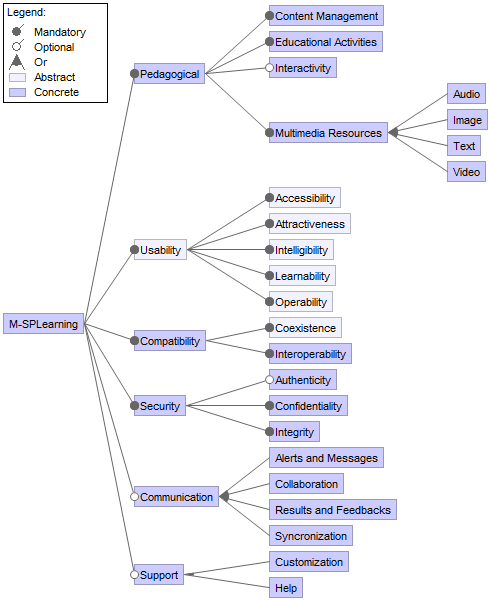
\includegraphics[scale=0.9]{figures/section3/MSPLFeatureModel}
    \caption{M-SPLearning Feature Model \cite{falvojr14a,falvojr14b}.}
    \label{figureMSPLFeatureModel}
\end{figure}

    %Engloba a coexistência e capacidade de trocar informações com outros sistemas no mesmo ambiente operacional. Por se mostrar essencial a aplicativos móveis, essas features foram definidas como obrigatórias.
    \item \textit{Compatibility}: include the coexistence and ability of a product to exchange information with other systems in a same operating environment. As they are essential for mobile applications, their features were defined as mandatory.
    
    %Trata-se de uma feature fundamental para qualquer aplicativo m-learning, uma vez que existem aspectos que devem ser garantidos para que os usuários confiem no produto gerado. As features que representam a integridade e confidencialidade foram definidas como obrigatórias devido a sua importância em termos de seguraça. Já a feature Authenticity é opcional porque nem todo aplicativo m-learning possui autenticação explícita de seus usuários.
    \item \textit{Security}: this is a key feature since any mobile application should send and receive data securely. Features \textit{Integrity} and \textit{Confidentiality} were defined as mandatory due to their importance in security terms. On the other hand, the \textit{Authenticity} feature is optional because not every m-learning application has explicit authentication of its users.
    
    %Provê o transporte de informações entre os usuários do aplicativo, possibilitando a troca de mensagens, a verificação resultados de testes e até mesmo a sincronização de atividades realizadas em outros dispositivos móveis. Essa feature é opcional e suas subfetaures possuem essa mesma definição, possibilitando qualquer combinação possível entre elas.
    \item \textit{Communication}: responsible for changing information among users of the application, enabling the exchanging of messages, testing results and synchronizing activities in other mobile devices. This feature and subfeatures are optional and accept any possible combinations.
    
    %Trata-se de uma feature considerada um diferencial de qualidade para os produtos em que ela está presente, pois provê alternativas de apoio ao usuário, como ajuda e internacionalização. Foi classificada como opcional por não ser um pré-requisito, assim como suas subfeatures.
    \item \textit{Support}: this feature provides some interesting alternatives to the user, as help and internationalization. All features and subfeatures was classified as an optional because it is not a prerequisite.
\end{itemize}

\subsubsection{Definition of Architecture}

%A partir do modelo de features apresentado anteriormente, definimos uma arquitetura de software aderente às necessidades do domínio educacional móvel. Tal arquitetura e seus respectivos componentes representam de forma abstrata os ativos centrais da M-SPLearning. Nesse sentido, a maioria das abordagens desenvolvidas para auxiliar no gerenciamento de variabilidades envolvem diversos conceitos e modelos de representação. A abordagem SMarty, em especial, é baseada na UML, amplamente aceita pela comunidade científica. Com isso, devido a sua facilidade de uso e resultados experimentalmente avaliados a SMarty foi escolhida para apoiar esta atividade da M-SPLearning.
From the feature model is necessary define an adherent software architecture to the mobile domain educational needs. Such an architecture and its components abstractly represent the core assets of M-SPLearning. Accordingly, most of the approaches developed to assist in the management of variability involve several concepts and representation models. SMarty, in particular, is based on UML, widely accepted by scientific and industrial communities. Due to its ease of use and results (experimentally evaluated), SMarty was chosen to support the design of the M-SPLearning promising architecture.

%A abordagem SMarty foi essencial durante todo o processo de desenvolvimento da LPS proposta, sobretudo por agregar seu perfil aos modelos UML para representação das similaridades e, principalmente, das variabilidades da M-SPLearning, como é o caso do diagrama de componentes arquiteturais ilustrado na Figura \ref{figureMSPLArchitecture}. Com base no diagrama arquitetural é possível identificar a base estrutural utilizada para a construção da M-SPLearning. O pacote com os ativos centrais engloba os componentes que representam as features definidas como concretas no modelo de features.
SMarty played an important role in the development of M-SPLearning, as it provided standards defined by the SMartyProfile to represent the similarities and, especially, the variabilities of M-SPLearning. The diagram of architectural components illustrated in Figure \ref{figureMSPLArchitecture} represents one of the diagrams developed with the support of SMarty. Based on the architectural diagram it is possible to identify the structural basis used to the construction of the M-SPLearning. The package \textit{Core Assets} comprises its concrete features as shown on Figure \ref{figureMSPLFeatureModel}.

\begin{figure}
    \centering
    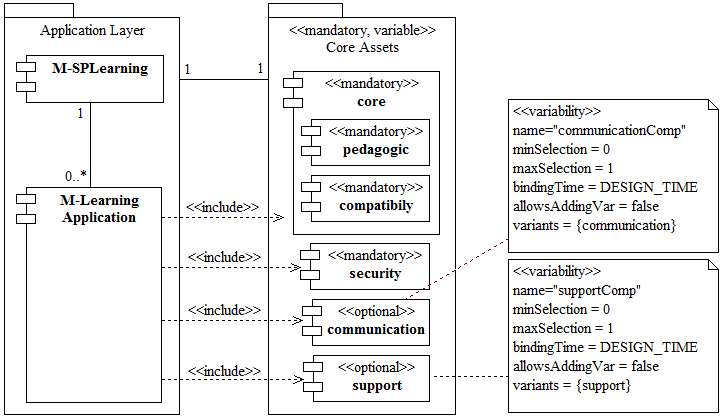
\includegraphics[scale=0.55]{figures/section3/MSPLArchitecture}
    \caption{M-SPLearning SMarty-based Architecture Diagram.}
    \label{figureMSPLArchitecture}
\end{figure}

%Os componentes que representam features específicas do domínio m-learning foram agrupados e nomeados como core. Assim, foi possível unificar os módulos fundamentais aos produtos gerados através da M-SPLearning. Além disso, é possível identificar alguns dos elementos da abordagem SMarty, que nesse caso representam as variabilidades em alto nível.
The components that represent the specific features of the m-learning domain were grouped into package \textit{core}. Therefore the fundamental modules for products generated by M-SPLearning. Could be unified and some of the elements of SMarty, representing the variabilities at a component level.

%A camada de aplicação, por sua vez, contém um componente que caracteriza a M-SPLearning, identificando sua associação com os ativos centrais e explicitando a possibilidade de criação de produtos, também representados como componentes. Cada produto gerado pode incluir as dependências disponíveis nos ativos centrais, fazendo com que cada produto possa utilizar dependências diferentes de acordo com as configurações definidas na M-SPLearning.
The \textit{Application Layer} contains a component that characterizes the M-SPLearning, identifying its association with core assets and enabling products derivation. Each product should include the components available in \textit{Core Assets}, making each m-learning application has different features according to your configurations defined in M-Learning.

\subsubsection{Components Design}

%Esta fase deve ser conduzida para projetar as variabilidades e similaridades identificadas pela Análise de Domínio. Nesse sentido, os componentes, arquitetonicamente armazenados junto aos ativos centrais, tiveram suas respectivas \textit{features} visualmente representadas por meio de um diagrama de componentes SMarty, ilustrado na Figura \ref{fig:msplDesign}.
In this phase are designed the variabilities and similarities identified in the Domain Analysis. Accordingly, the core assets elements were visually represented by SMarty diagram components (Figure \ref{figureMSPLDesign}).

\begin{figure}
\centering
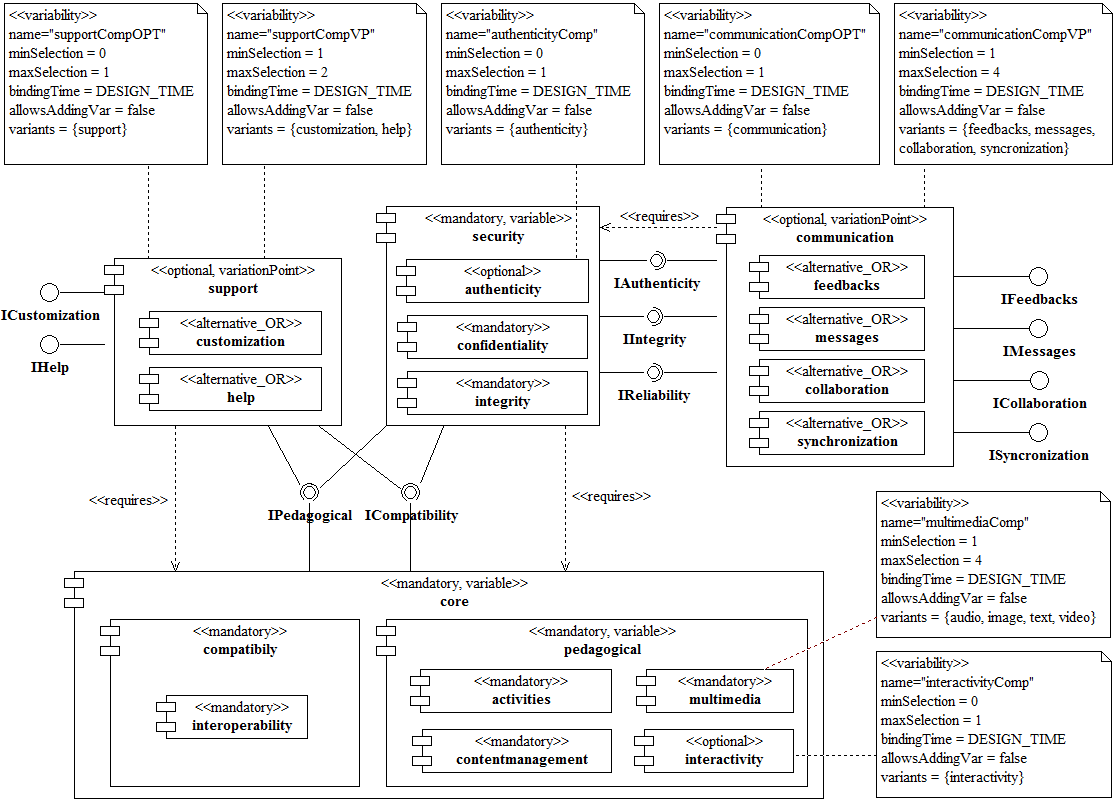
\includegraphics[scale=0.445]{figures/section3/MSPLDesign}
\caption{M-SPLearning SMarty-based Components Diagram.}
\label{figureMSPLDesign}
\end{figure}

%Por meio desse diagrama de componentes é possível visualizar todas as features concretas contempladas pela M-SPLearning. Os componentes resultantes foram rotuladas com os estereótipos característicos da abordagem SMarty. Esse diagrama permite a analise da quantidade de configurações possíveis aos aplicativos m-learning contemplados pela LPS.
The diagram shows all concrete features covered by M-SPLearning. The resulting components are labeled with the characteristic stereotypes of SMarty approach. This diagram presents the possible component configurations, based on features, for m-learning applications covered by the SPL.
%Por exemplo, o componente multimedia foi modelado como uma variabilidade (esteriótipo variability), ou seja, ele pode ser configurado para que uma LPS crie aplicações m-learning customizadas de acordo com suas configurações. Dessa forma, uma aplicação poderia ser configurada para possuir no mínimo um e no máximo quatro recursos multimédia (audio, image, text e video), conforme as notações "minSelection" e "maxSelection". Uma observação relevante é que qualquer componentes cujo filho foi modelado como uma variabilidade deve ser marcado como variável (esteriótipo variable).
For example, the \textit{multimedia} component was modeled with variability stereotype, i.e., the SPL can be configured for create custom m-learning applications with such features. Therefore, a product can be configured so as to between have one and four \textit{multimedia} resources (audio, image, text and video), according to notations ``minSelection" and ``maxSelection". Any component formed for other components with variability should be tagged with the variable stereotype.

% 30/12/2015 03:02 %

%Com ênfase no domínio explorado, os componentes pedagogical e communication se destacam, assim como seus requisitos. Nesse sentido, a maioria dos componentes pedagógicos são obrigatórios, com variabilidades possíveis em termos de interatividade e recursos multimídia (já explanada anteriormente). Por sua vez, os componentes agrupados em communication são alternativos, sendo que ao menos um deles deve agregar sua funcionalidade aos produtos gerados.
With emphasis on the explored domain, the \textit{pedagogical} and \textit{communication} components stand out, as well as your requirements. In this sense, most \textit{pedagogical} subcomponents are mandatory, with possible variabilities in terms of \textit{interactivity} and \textit{multimedia} features, whereas the \textit{communication} subcomponents are alternative, and at least one of them must provide its functionalities to the generated products.

%Também fica explícito o relacionamento de dependência entre os componentes modelados. Como definido anteriormente, o componente core unifica as features integralmente obrigatórias ao domínio m-learning, tornando-se necessário, direta ou indiretamente, aos componentes security, communication e support. A particularidade aqui fica por conta do componente communication, dependente do componente security, que por sua vez está relacionado com o componente core, fazendo com que o componente communication também tenha acesso a essa dependência. Isso garante a imposição arquitetônica de que todos os componentes parcialmente mandatórios ou opcionais dependam do componente core, que proverá as características fundamentais da M-SPLearning.
The dependency relationship between the modeled components can also be observed. As previously defined, the \textit{core} component unifies the mandatory features for the m-learning domain, being necessary, directly or indirectly, to the \textit{security}, \textit{communication} and \textit{support} components. Particularly, the \textit{communication} component depends on the \textit{security} component, which is related to the \textit{core} component. As a consequence, the \textit{communication} component also knows the \textit{core}.

%A partir do Projeto de Componentes aferidos pela LPS, torna-se possível a definição de um Plano de Produção que transforme as representações abstratas em produtos de software concretos, com suas respectivas variabilidades. A seção a seguir conclui a Análise de Domínio definida para a M-SPLearning.
Through Components Project it is possible to define a Production Plan to transform the abstract representations in concrete software products, with their respective variabilities, as following.

\subsubsection{Production Plan}

%O Plano de Produção prescreve como os produtos devem ser gerados a partir dos ativos centrais definidos para a LPS. Para isso, um diagrama de atividades usando a abordagem SMarty foi modelado, expondo as variabilidades possíveis durante o processo de criação de um produto (Figura \ref{figureMSPLProductionPlan}). Basicamente, este plano pode ser considerado um ativo central da M-SPLearning, assim como qualquer outro artefato que contribua para a criação sistemática de seus produtos. 
The Production Plan prescribes how the products should be generated from the core assets identified for the SPL. An activity diagram using the SMarty approach and exposing the possible variabilities in the creation of a product (Figure \ref{figureMSPLProductionPlan}) was modeled. Basically, this plan can be considered a core asset of M-SPLearning, as any other artifact that contributes to the systematic creation of its products.

\begin{figure}
\centering
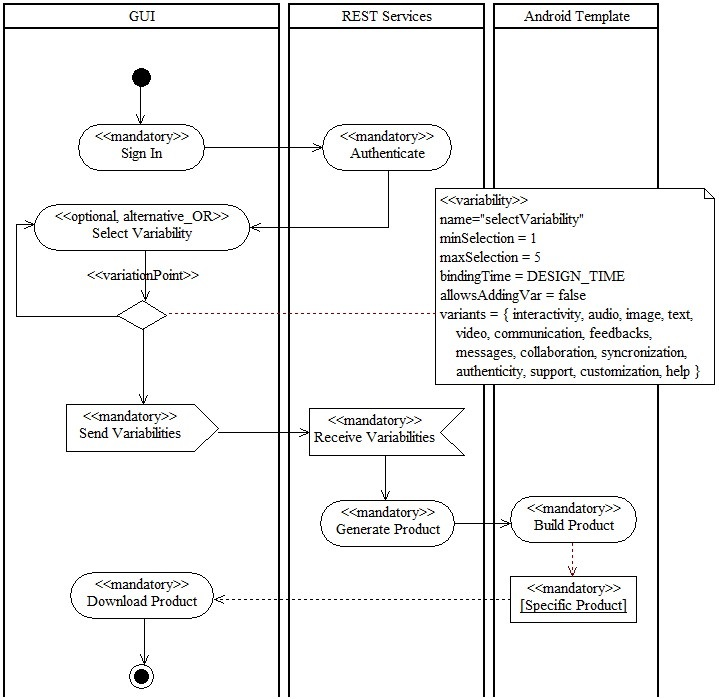
\includegraphics[scale=0.4]{figures/section3/MSPLProductionPlan}
\caption{M-SPLearning SMarty-based Production Plan.}
\label{figureMSPLProductionPlan}
\end{figure}

%O ponto de variação definido no plano de produção expõe todas as variabilidades elicitadas para a M-SPLearning. Desta forma, a customização dos produtos foi centralizada em um único ponto, agilizando o processo de configuração e geração dos aplicativos m-learning, provenientes da LPS proposta.
The variation point defined in the production plan exposes all variabilities elicited for M-SPLearning. Therefore, the customization of the products was centralized at a single point and streamlined the configuration process and generation of m-learning applications by the SPL proposal.

%Cada raia do diagrama representa um módulo específico, sendo possível identificar algumas características arquiteturais da M-SPLearning. Uma das mais importantes neste sentido é a utilização do conceito de REpresentational State Tranfer (REST). Essa característica permite a criação e consumo de web services por meio do padrão Hypertext Transfer Protocol (HTTP), tornando viável a utilização de arquiteturas emergentes, como a Service-Oriented Architecture (SOA), também no contexto de aplicações móveis.
Each swimlane of the diagram represents a specific module, and enables identification of some architectural characteristics of the M-SPLearning. One important point is the use of the REpresentational State Transfer (REST) \cite{fielding00} architectural style. Through this concept, web services can be created and consumed by the Hypertext Transfer Protocol (HTTP) and emerging software architectures, as Service-Oriented Architecture (SOA) can be used also in the context of mobile applications.

%A seguir cada módulo representado no diagrama de atividades é sintetizado, considerando suas características técnicas e responsabilidades em termos práticos:
Each module represented in Figure \ref{figureMSPLProductionPlan} is synthesized according to its main characteristics in technical terms:

\begin{itemize}
    %Módulo que provê a interface gráfica dos usuários da LPS, ou seja, as representações visuais com as quais os usuários interagem para a geração dos produtos apoiados pela M-SPLearning. Neste módulo, é possível configurar as variabilidades e visualizar as similaridades, além de solicitar a geração de um produto personalizado. Este módulo foi implementado utilizando apenas tecnologias client-side, em especial HTML, JavaScript e CSS. A ideia foi demonstrar a interoperabilidade em uma arquitetura SOA, já que foram implementados todos os serviços usando REST, conforme o item a seguir.
	\item \textbf{\textit{Graphical User Interface (GUI):}} a module that provides the visual representations with which users interact to generate the products supported by M-SPLearning. Variabilities can be configured for the generation of a customized product. This module was implemented through client-side technologies, especially HTML, JavaScript and CSS. The idea was to demonstrate interoperability in a SOA architecture, since all services were implemented using REST.
	
	%Módulo desenvolvido a partir da abstração arquitetônica REST, que se caracteriza pelo uso de tecnologias e protocolos da web para a criação e entrega de serviços. Este estilo é totalmente aderente ao padrão arquitetural SOA e assegura a disponibilidade e consumo de web services de uma forma simples e eficiente. Este módulo corresponde à principal interface entre os produtos gerados pela M-SPLearning e suas features. Ele acessa um banco de dados remoto, onde todas as informações são armazenadas, incluindo as features (similaridades e variabilidades) especificadas via GUI. A centralização dos dados no módulo de serviços torna-o essencial para os outros (GUI e Android Template), uma vez que ambos consomem os web services disponibilizados por ele.
	\item \textbf{\textit{REST Services:}} a module developed from the REST architectural abstraction and characterized by the use of technologies and protocols of the web for the creation and delivery of services. This style is fully adherent to the SOA architectural pattern and ensures the availability and consumption of web services in a simple and efficient way. It is the main interface between the products generated by the M-SPLearning and their features and accesses a remote database where all the information is stored, including features (similarities and variabilities) configured from the \textit{GUI}. The centralization of data in the \textit{REST Services} module is essential for other modules (\textit{GUI} and \textit{Android Template}), since both consume the web services provided.
	
	%Este módulo provê um template genérico para a customização dos produtos. Isso permite que um serviço, disponível no módulo REST Services, execute uma compilação personalizada de acordo com as variabilidades configurados no módulo GUI. O resultado é um Android Application Package (APK) com todas as features pré-configuradas, o que permite a instalação do produto customizado em qualquer dispositivo Android.
	\item \textbf{\textit{Android Template:}} a module that provides a generic template for the customization of products. Therefore, the \textit{REST Services} module executes a custom build, according to the variabilities configured in the \textit{GUI}. The result is an Android Application Package (APK) with all pre-configured features for the installation of a custom product on any Android device.
\end{itemize}

%Considerando a necessidade de construção de aplicações m-learning com maior qualidade e reúso, os esforços para o desenvolvimento de LPS que lidam com aspectos SOA ganharam especial importância no contexto móvel. A adoção de uma abordagem SOA torna-se cada vez mais relevante, principalmente porque torna mais fácil e flexível a construção de suas aplicações, promovendo interoperabilidade e reutilização, o que corrobora com as definições arquiteturais propostas no plano de produção.
Considering the need of building m-learning applications with higher quality and reuse, efforts for the development of SPL dealing with SOA aspects gained special importance in the mobile context \cite{marinho10,nascimento11}. The adoption of an SOA approach has become increasingly important, especially because its applications are easy and flexible and promote interoperability and reuse, which agrees with the architectural definitions proposed in the production plan.

%A M-SPLearning foi elaborada a partir de um processo baseado em práticas e conceitos relevantes no âmbito da Engenharia de Software. Com isso, a M-SPLearning utilizou um processo sequencial para sua definição, abordando as dificuldades da análise de elementos do domínio e as definições arquiteturais necessárias para sua implementação proativa. A próxima seção trata da atividade primária subsequente, a Engenharia de Aplicação.
M-SPLearning was elaborated from a process based on relevant practices and concepts in software engineering and has used an incremental process for its definition, addressing the difficulties of domain analysis and the architectural definitions necessary for a proactive implementation. The next section addresses the subsequent SPL activity, i.e., the AE.

\subsection{Application Engineering}\label{section32}

%Esta atividade depende essencialmente dos artefatos de saída da Engenharia de Domínio, que agora atuam como artefatos de entrada. A partir dos ativos gerados, um conjunto específico de features foi selecionado para a implementação da M-SPLearning. Essa redução de escopo foi definida com o objetivo de viabilizar a avaliação experimental da M-SPLearning. Dessa forma, com um número reduzido de features, foi possível implementar e avaliar a LPS em um prazo aceitável.
This activity depends on the output artifacts of DE, which now act as input devices. A specific set of features with such artifacts was selected for the implementation of M-SPLearning. This reduction in scope was defined for an experimental evaluation of the M-SPLearning. Therefore, the SPL could be implemented with a limited number of features in 188 hours, which enabled their experimental evaluation.

%No contexto deste trabalho, as features relacionadas às atividades pedagógicas e de segurança foram priorizadas e implementadas. O motivo dessa escolha é que as features em questão representam os requisitos funcionais mínimos de uma aplicação m-learning, são eles: (i) Pedagogical: inclui a realização de atividades educacionais através do gerenciamento de conteúdos interativos e recursos multimédia; (ii) Security: agrega em termos de confidencialidade e integridade dos dados, além da possibilidade de autenticação dos usuários; e (iii) Communication: incluiu apenas a feature relacionada à sincronização de dados.
In this study features related to teaching and security activities were prioritized and implemented because they are the minimum functional requirements of an m-learning application: (i) \textit{Pedagogical}: includes educational activities through the management of interactive and multimedia content; (ii) \textit{Security}: provides confidentiality and integrity of data, which includes the user authentication; and (iii) \textit{Communication}: includes features related to data synchronization.

%Tecnicamente, a M-SPLearning apresenta a visão lógica de uma LPS definida para configuração e geração de aplicações m-learning na plataforma Android. Sua implementação foi feita predominantemente em Java e seu código fonte pode ser consultado a partir do repositório open source GitHub.
In technical terms,  M-SPLearning shows a logical view of an SPL defined for configuration and generation of m-learning applications on the Android platform. It was implemented predominantly in Java and its source code is available\footnote{http://github.com/falvojr/msplearning} in GitHub open source repository.

%Por definição, a Engenharia de Aplicação instancia os ativos centrais de uma LPS para geração de produtos específicos. Para isso, o plano de produção, até então abstrato, foi utilizado para a construção de seus respectivos módulos concretos. No contexto desta atividade, o módulo GUI foi inevitavelmente o mais explorado, porque todos os produtos são gerados através dele.
By definition, the AE instantiates the core assets of SPL to generate specific products. The production plan was used for the construction of the respective concrete modules. In such an activity, the \textit{GUI} module is inevitably the most exploited, because all products are generated through it.

%A primeira interação entre usuário e a M-SPLearning ocorre em uma página inicial web. Nela, os usuários podem registrar-se e, posteriormente, autenticar-se na aplicação. Essa interface visual também introduz o domínio e os principais objetivos da M-SPLearning, contextualizando seus usuários. Outro aspecto relevante foi a construção de suas páginas web completamente baseadas no conceito de layouts responsivos, o que, dentre outras tendências, tornou a representação visual da LPS ainda mais dinâmica e flexível. A Figura \ref{figureMSPLWebLogin} expõe tais características.
The first interaction between the user and M-SPLearning occurs in a web home page. Users can sign up and access the application. This interface also introduces the domain and the main objectives of M-SPLearning. Another important aspect refers to the construction of the web pages completely based on the concept of responsive layouts, which makes the visual representation of SPL even more dynamic and flexible. 

%Figure \ref{figureMSPLWebLogin} presents such characteristics.
%
%\begin{figure}
%\centering
%\includegraphics[scale=0.4]{figures/section3/MSPLWebLogin}
%\caption{M-SPLearning GUI Login.}
%\label{figureMSPLWebLogin}
%\end{figure}

%Com um usuário devidamente autenticado, a interface resultante é a caracterização mais evidente da M-SPLearning, já que possibilita o gerenciamento visual das variabilidades disponibilizadas pela LPS. Neste ponto, o usuário, por exemplo um professor, simplesmente realiza alguns cliques para geração de um produto específico, criando, assim, um APK com uma aplicação m-learning instalável em qualquer dispositivo Android.
With an authenticated user, the resulting interface represents the M-SPLearning, as it enables the visual management of all variabilities provided by SPL. At this point, the user, for example a teacher, simply performs a few clicks to generate a specific product that creates an APK that encapsulates a custom m-learning application for any Android device. The page for this procedure is illustrated in Figure \ref{figureMSPLWebGeneration}, which also shows the visual interface for the management of products generated by M-SPLearning. Furthermore, variabilities related to features prioritized during this implementation can be configured in the products generation.

%A página para a realização desse procedimento é ilustrado pela Figura 1, que também apresenta a interface visual para o gerenciamento dos produtos gerados através da M-SPLearning. Além disso, é importante observar que as variabilidades relacionadas às features priorizadas durante essa implementação podem ser configuradas na geração dos produtos.

\begin{figure}
\centering
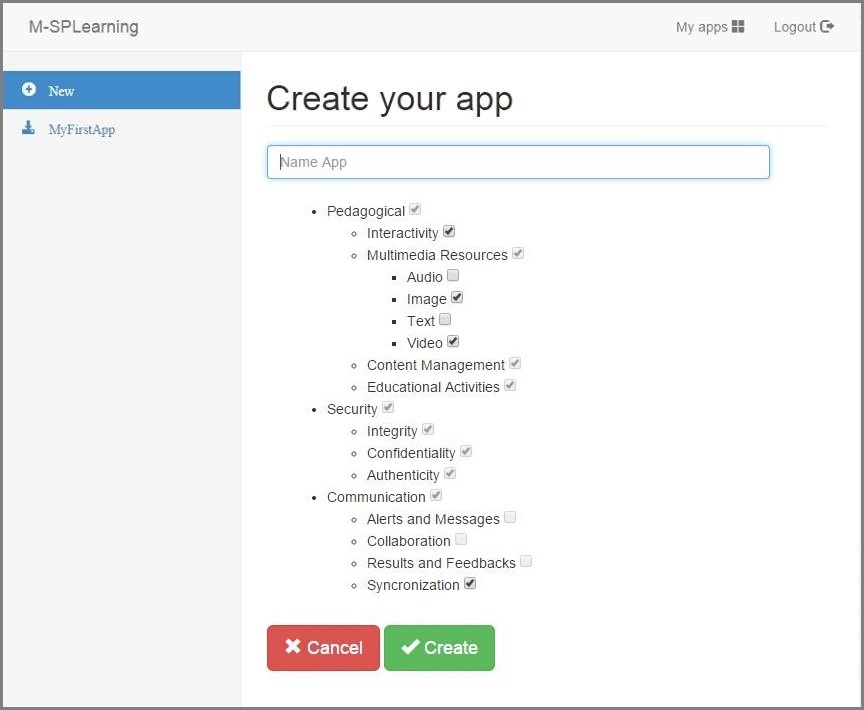
\includegraphics[scale=0.4]{figures/section3/MSPLWebGeneration}
\caption{M-SPLearning GUI Product Generation.}
\label{figureMSPLWebGeneration}
\end{figure}

%Ao solicitar a geração de um APK, os módulos REST Service e Android Template são acionados simultaneamente. Essa integração resulta na criação de um produto aderente às variabilidades selecionadas pelo usuário. A partir deste momento a aplicação m-learning gerada pode ser instalada no dispositivo móvel de qualquer professor ou aluno, que deve se registrar na aplicação móvel, caso a feature Authentication tenha sido selecionada durante a criação do APK.
When the generation of as APK is required, the \textit{REST Services} and \textit{Android Template} modules are triggered simultaneously. This integration results in the creation of an adherent product for user's selected variabilities. The m-learning application generated can be installed in the Android device of any teacher or student, who must register with the mobile application if feature \textit{Authentication} has been selected in the creation of the APK.

%A Figura 1 mostra dois produtos gerados com as variabilidades Authenticity e Interactivity configuradas de formas diferentes, nas quais: (a) o produto foi configurado apenas com a feature Authenticity; e (b) o produto foi gerado com ambas as variabilidades, o que explica o formulário de autenticação com a possibilidade de interação com algumas redes sociais.
Figure \ref{figureMSPLLogin} shows two products generated with \textit{Authenticity} and \textit{Interactivity} variabilities configured in different ways: (a) the product was configured with only the Authenticity feature; and (b) the product was generated with both variabilities, which explains the authentication form with the possibility of interaction with some social networking.

\begin{figure}
\centering
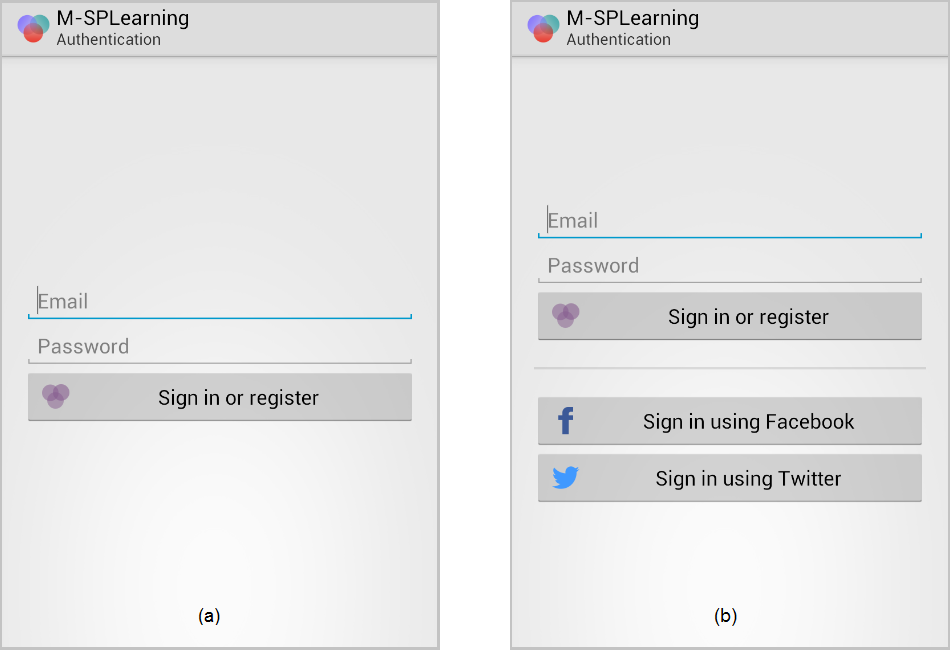
\includegraphics[scale=0.33]{figures/section3/MSPLLogin}
\caption{M-SPLearning Product Login -- Configurations of the features:\newline(a) \textit{Authenticity}; and (b) \textit{Authenticity} and \textit{Interactivity}.}
\label{figureMSPLLogin}
\end{figure}

%Observando a Figura 1 nota-se que o botão comum aos produtos também prevê a possibilidade de registro de um novo usuário. Para isso, o usuário deve apenas preencher seu e-mail e senha nos campos disponíveis para que a aplicação m-learning verifique a existência de seu usuário. Em caso negativo, o formulário de cadastro é exibido já com as informações digitadas preenchidas (Figura 2).
According to Figure \ref{figureMSPLLogin}, the common button for products also provides the possibility of registering. For this, the user should fill his/her email and password in the fields available for the application to verify if the user exists (Figure \ref{figureMSPLRegister} (a)). If not, the registration form is displayed with the information previously typed (Figure \ref{figureMSPLRegister} (b)).

\begin{figure}
\centering
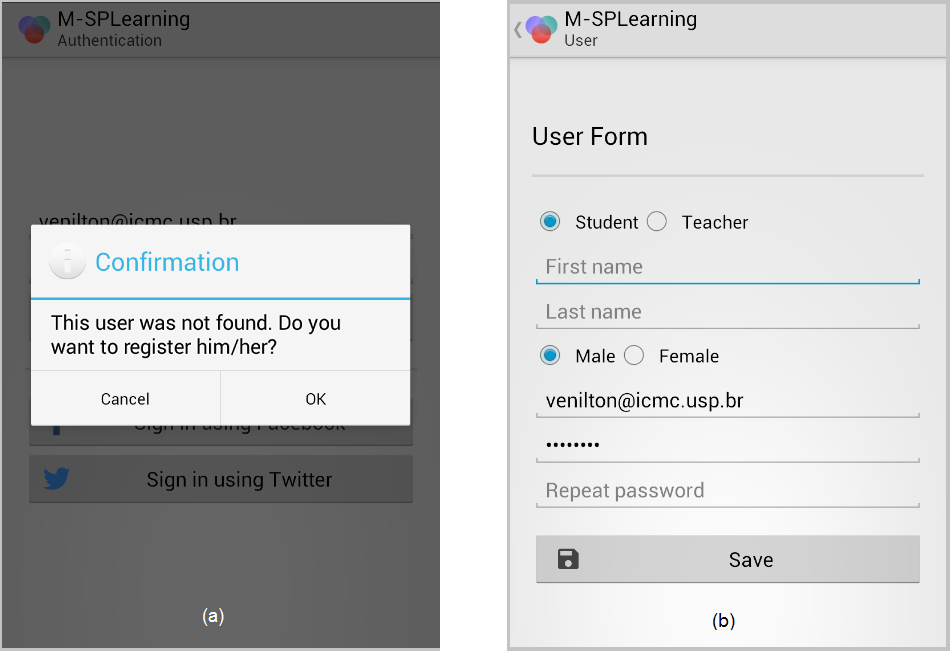
\includegraphics[scale=0.33]{figures/section3/MSPLRegister}
\caption{M-SPLearning Product Registration -- Steps for user registration:\newline(a) Confirmation message; and (b) Registration Form.}
\label{figureMSPLRegister}
\vspace{0.65cm}
\end{figure}

%O formulário de cadastro de usuário permite a seleção do tipo de acesso: professor ou aluno. Por motivos de segurança, todos os usuários registrados devem ser aprovados pelo usuário que gerou o APK. Para isso, no momento de criação da aplicação o usuário é associado a mesma com perfil administrativo. Esse aspecto deixa evidente a feature "Content Management", uma vez que cada perfil de usuário prevê acessos específicos e bem definidos. A Figura 1 ilustra um cenário possível, em que: (a) apresenta a visão de um professor; e (b) apresenta a visão de um aluno, com o adendo de que neste exemplo nenhum conteúdo educacional foi incluído, tendo em vista que o acesso a esta funcionalidade está desabilitado.
A user can select the type of access, teacher or student in the registration form. For security reasons, all registered users must be approved by the user who generated the APK. At the time of the APK creation the user is associated with an administrative profile. This aspect clarifies feature \textit{Content Management}, since each user's profile provides specific and well-defined accesses. Figure \ref{figureMSPLDashboardApp} illustrates a possible scenario with (a) teacher's views and (b) student's view, but with no content, since the access to this feature is disabled.

\begin{figure}
\centering
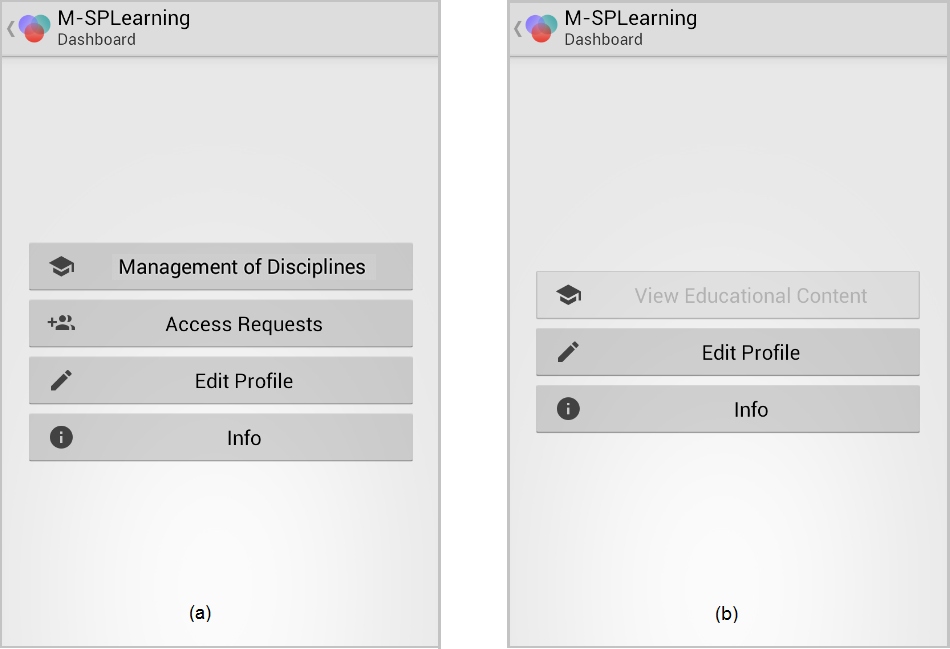
\includegraphics[scale=0.34]{figures/section3/MSPLDashboardApp}
\caption{M-SPLearning Product Dashboard -- Access Profiles:\newline(a) Teacher; and (b) Student.}
\label{figureMSPLDashboardApp}
\end{figure}

%Com um usuário devidamente autenticado e com suas respectivas funcionalidades fornecidas, a aplicação m-learning está pronta para armazenamento e compartilhamento do seu principal ativo, os conteúdos educacionais. Neste sentido, o professor pode cadastrar suas disciplinas, lições e finalmente o conteúdo de cada uma delas. Essas funcionalidades representam um contexto de uso das features Educational Activities e Multimedia Resources, também representadas pela Figura 1.
After the user has been properly authenticated, the m-learning application is ready for storage and sharing of its main asset, i.e., the educational content. The teacher can register his/her courses, lessons and finally the content of each lesson. These functionalities are a usage sample of the \textit{Educational Activities} and \textit{Multimedia Resources} shown in Figure \ref{figureMSPLEducationalContent}.

\begin{figure}
\centering
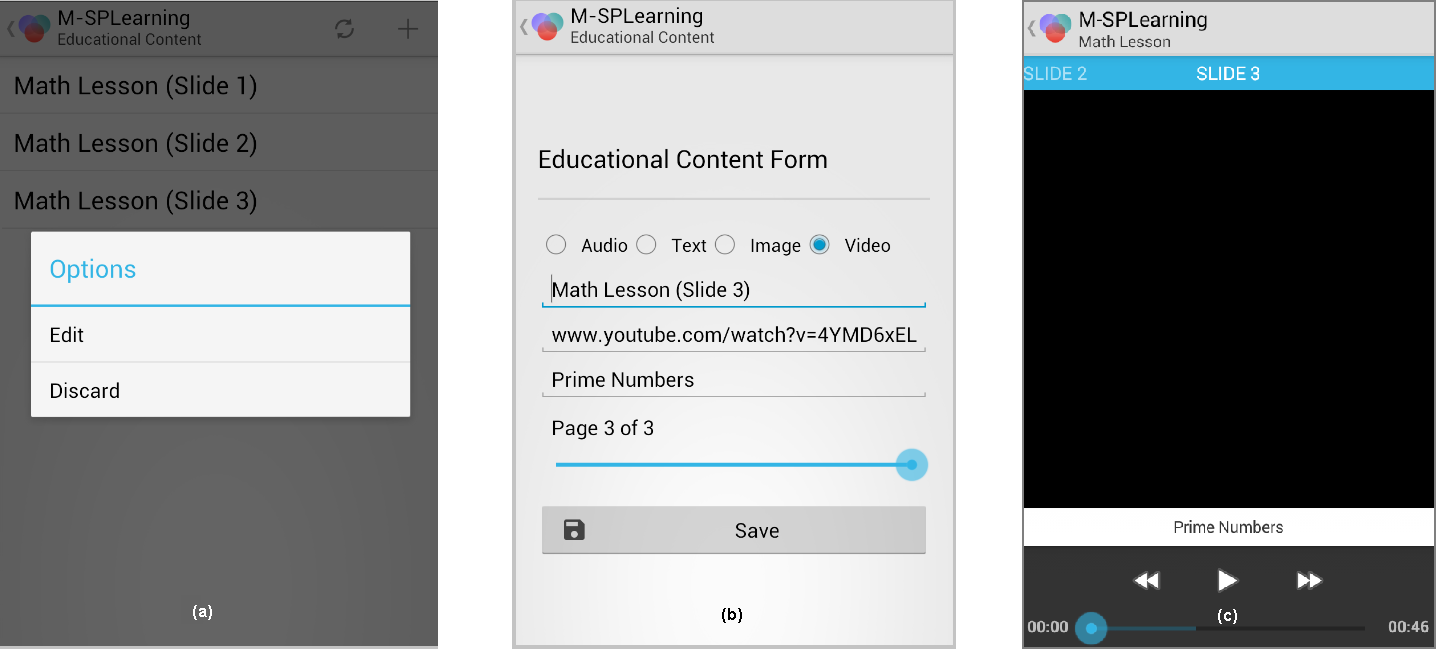
\includegraphics[scale=0.34]{figures/section3/MSPLEducationalContent}
\caption{M-SPLearning Product Educational Content Management:\newline(a) Listing of educational content and context menu; (b) Editing form; and (c) Displaying video content.}
\label{figureMSPLEducationalContent}
\end{figure}

%De acordo com as features disponibilizadas pela M-SPLearning, nota-se a possibilidade de inclusão de conteúdos educacionais dos seguintes tipos: áudio, texto, imagem e vídeo. No exemplo apresentado, a opção de vídeo está selecionada, o que provê ao professor a inclusão de uma URL para a disponibilização do vídeo desejado aos alunos que compartilham essa aplicação.
According to the features provided by M-SPLearning as audio, text, image and video can be included. %In the example shown, the video is selected, providing to the teacher the inclusion of an URL to the availability of the desired video students to share this application.
%Assim, os alunos visualizam os conteúdos educacionais incluídos pelos professores cadastrados na aplicação, obtendo assim acesso centralizado a sua gama de conteúdos educacionais. A Figura 1 ilustra, na perspectiva de aluno, um exemplo de conteúdo educacional do tipo vídeo.
Figure \ref{figureMSPLEducationalContent} (c) illustrates an example of a video feature from a student perspective.

%É importante observar que foi possível incluir os requisitos previamente definidos para a construção de uma LPS. A concepção da M-SPLearning envolveu desde a análise e projeto até a implementação funcional da proposta desta pesquisa. A avaliação formal da M-SPLearning, junto de sua abordagem e principais resultados, são descritos na Seção \ref{section4}.
The requirements previously set for the construction of an SPL can also be included. The design of the M-SPLearning involved from analysis and design to functional implementation. A formal evaluation of the M-SPLearning, along with this approach and main results is described in Section \ref{section4}.

% 30/12/2015 06:22 %

\section{M-SPLear\allowbreak ning Experimental Evaluation}\label{section4}

This section reports the experimental evaluation of M-SPLear\allowbreak ning regarding time-to-market and quality improvement. M-SPLear\allowbreak ning was compared with a software singular development methodology. The guidelines proposed by Jedlitschka et al. \cite{jedlitschka07} were followed for controlled experiments.

\subsection{Motivation}\label{sub:motivation}


The choice for the adoption of new technologies or approaches used in the development process depends on several aspects of quality and benefits. Although many approaches have been developed, many issues about them must be solved for a suitable adoption in both industry and academic environments. Experimental evaluations may shed light on the identification of evidences from quality and benefits of an approach, justifying their choice. In some cases, the collected evidence may still support the correction of problems identified during the experimental evaluations and improvements in the proposals \cite{wohlin12,juristo10}.

Therefore, the experimental evaluation of the M-SPLear\allowbreak ning is presented based on two relevant software development variables: time-to-market and number of faults.

\subsubsection{Research Objectives}\label{sub:object}

The experiment aimed at a \textbf{comparison} between the singular software development (SSD) and the software product line (SPL) methodologies, \textbf{for the purpose of} identification of the most efficient, \textbf{regarding} the time spent on the creation of software products (time) and number of their faults, \textbf{in the context of} practitioners from industry.


\subsection{Experimental Design}\label{sub:design}

This section describes the experimental design and procedures for support of future replications.

\subsubsection{Goals}

Two research questions (R.Q.) based on the research objective were raised:

\textbf{R.Q.1} Which methodology is more efficient regarding time-to-market, SSD or SPL?

\textbf{R.Q.2} Which methodology showed more quality in terms of number of faults in the software product created, SSD or SPL?

\subsubsection{Hypotheses}

Two sets of hypotheses were defined to be tested and each of them is related to its respective research questions (R.Q.1 and R.Q.2):

\textbf{R.Q.1 hypotheses:} time-to-market

	\begin{itemize}
	
	\item \textbf{Null Hypothesis ($H_{0}$)}: there is no significant difference of time-to-market between SSD and SPL.
	
	$H_{0}$ : $\mu$(\textit{t(SSD)}) =  $\mu$(\textit{t(SPL)});
	
	\item \textbf{Alternative Hypothesis ($H_{1}$)}: SSD has less time-to-market than SPL.
	
	$H_{1}$ : $\mu$(\textit{t(SSD)}) $<$ $\mu$(\textit{t(SPL)});
		
	
	\item \textbf{Alternative Hypothesis ($H_{2}$)}: SSD has more time-to-market than SPL.
	
	$H_{2}$ :  $\mu$(\textit{t(SSD)}) $>$ $\mu$(\textit{t(SPL)}).		
	
	\end{itemize}	

\textbf{R.Q.2 hypotheses:}
quality in terms of number of faults
	\begin{itemize}
	
	\item \textbf{Null Hypothesis ($H_{0}$)}: there is no significant difference between SSD and SPL with regard to quality regarding number of faults in the software products created.
	
	$H_{0}$ : $\mu$(\textit{d(SSD)}) =  $\mu$(\textit{d(SPL)});
	
	\item \textbf{Alternative Hypothesis ($H_{1}$)}: SSD has a larger number of faults than SPL.
	
	$H_{1}$ : $\mu$(\textit{d(SSD)}) $>$ $\mu$(\textit{d(SPL)});
		
	\item \textbf{Alternative Hypothesis ($H_{2}$)}: SSD has a smaller number of faults than SPL.
	
	$H_{2}$ :  $\mu$(\textit{d(SSD)}) $<$ $\mu$(\textit{d(SPL)}).		
	
	\end{itemize}

\subsubsection{Variables}

Dependent variables are the mean of time ($t$) and faults ($f$), defined as follows:

\small

\begin{equation}\label{eq:1}
\mu{(t)}=(\Sigma xi)/n, i = 1..n
\end{equation}
\begin{equation}\label{eq:2}
\mu{(f)}=(\Sigma yi)/n, i = 1..n
\end{equation}
\normalsize 
where:
\begin{itemize}
\item \textit{t} is the implementation time (minutes);
\item \textit{f} is the number of faults;
\item \textit{xi} is the time of implementation of participant i;
\item \textit{yi} is the number of faults detected in the implementation of participant i; and
\item \textit{n} is the total of participants in the experiment.
\end{itemize}
\normalsize

Independent variables are the development methodology, which is a factor with two treatments (SSD and SPL), and the software product configuration for mobile learning platform, which is a factor with two treatments namely product 1 (P1) and product 2 (P2). Table \ref{tab:variables} shows the description of dependent and independent variables.

%\begin{landscape}

\begin{table}
\centering
\caption{\label{tab:variables}Dependent and Independent Variables Description.}
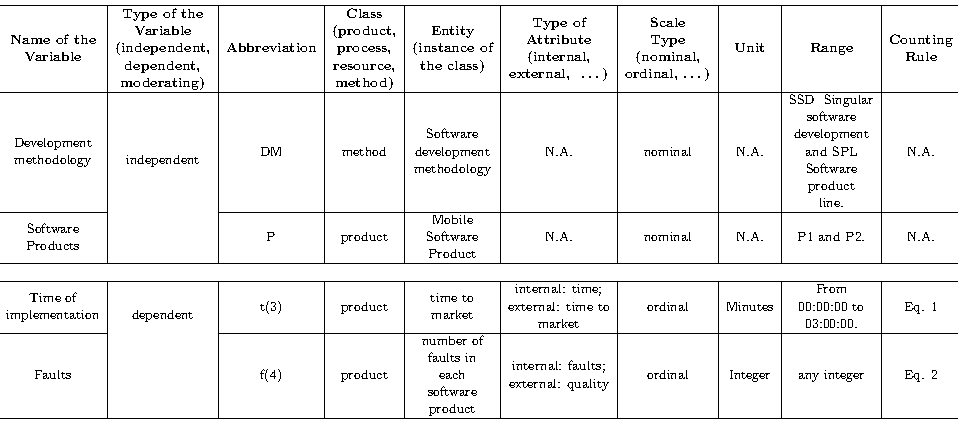
\includegraphics[scale=0.75]{figures/section4/tab_n.pdf}



%\resizebox{1.2\textwidth}{!}{
%\small
%\begin{tabular}{cccccccccc}
%\multicolumn{1}{l}{}                                                                         & \multicolumn{1}{l}{}                                                                                                                      & \multicolumn{1}{l}{}                                 & \multicolumn{1}{l}{}                                                                                                        & \multicolumn{1}{l}{}                                                                                           & \multicolumn{1}{l}{}                                                                                                        & \multicolumn{1}{l}{}                                                                                            & \multicolumn{1}{l}{}                                                                & \multicolumn{1}{l}{}                                                                                                                             & \multicolumn{1}{l}{}                                              \\ \hline
%\multicolumn{1}{c|}{\textbf{\begin{tabular}[c]{@{}c@{}}Name of the\\ Variable\end{tabular}}} & \multicolumn{1}{c|}{\textbf{\begin{tabular}[c]{@{}c@{}}Type of the\\ Variable\\ (independent, \\ dependent, \\ moderating)\end{tabular}}} & \multicolumn{1}{c|}{\textbf{Abbreviation}}           & \multicolumn{1}{c|}{\textbf{\begin{tabular}[c]{@{}c@{}}Class\\ (product, \\ process, \\ resource, \\ method)\end{tabular}}} & \multicolumn{1}{c|}{\textbf{\begin{tabular}[c]{@{}c@{}}Entity\\ (instance of \\ the class)\end{tabular}}}      & \multicolumn{1}{c|}{\textbf{\begin{tabular}[c]{@{}c@{}}Type of \\ Attribute \\ (internal, \\ external, \ \ldots)\end{tabular}}} & \multicolumn{1}{c|}{\textbf{\begin{tabular}[c]{@{}c@{}}Scale\\  Type \\ (nominal, \\ ordinal,\ \ldots)\end{tabular}}} & \multicolumn{1}{c|}{\textbf{Unit}}                                                  & \multicolumn{1}{c|}{\textbf{Range}}                                                                                                              & \textbf{\begin{tabular}[c]{@{}c@{}}Counting \\ Rule\end{tabular}} \\ \hline
%\multicolumn{1}{c|}{\begin{tabular}[c]{@{}c@{}}Development\\ methodology\end{tabular}}       & \multicolumn{1}{c|}{\multirow{2}{*}{independent}}                                                                                         & \multicolumn{1}{c|}{DM}                              & \multicolumn{1}{c|}{method}                                                                                                 & \multicolumn{1}{c|}{\begin{tabular}[c]{@{}c@{}}Software\\ development \\ methodology\end{tabular}}             & \multicolumn{1}{c|}{N.A.}                                                                                                   & \multicolumn{1}{c|}{nominal}                                                                                    & \multicolumn{1}{c|}{N.A.}                                                           & \multicolumn{1}{c|}{\begin{tabular}[c]{@{}c@{}}SSD – Singular \\ software \\ development \\ and SPL \\ Software \\ product\\  line.\end{tabular}} & N.A.                                                              \\ \cline{1-1} \cline{3-10} 
%\multicolumn{1}{c|}{\begin{tabular}[c]{@{}c@{}}Software\\ Products\end{tabular}}             & \multicolumn{1}{c|}{}                                                                                                                     & \multicolumn{1}{c|}{P}                               & \multicolumn{1}{c|}{product}                                                                                                & \multicolumn{1}{c|}{\begin{tabular}[c]{@{}c@{}}Mobile\\ Software \\ Product\end{tabular}}                      & \multicolumn{1}{c|}{N.A.}                                                                                                   & \multicolumn{1}{c|}{nominal}                                                                                    & \multicolumn{1}{c|}{N.A.}                                                           & \multicolumn{1}{c|}{P1 and P2.}                                                                                                                  & N.A.                                                              \\ \hline
%\multicolumn{10}{c}{}                                                                                                                                                                                                                                                                                                                                                                                                                                                                                                                                                                                                                                                                                                                                                                                                                                                                                                                                                                                                                                                                                       \\ \hline
%\multicolumn{1}{c|}{\begin{tabular}[c]{@{}c@{}}Time of \\ implementation\end{tabular}}       & \multicolumn{1}{c|}{\multirow{2}{*}{dependent}}                                                                                           & \multicolumn{1}{c|}{\begin{equation}t\end{equation}} & \multicolumn{1}{c|}{product}                                                                                                & \multicolumn{1}{c|}{\begin{tabular}[c]{@{}c@{}}time to\\ market\end{tabular}}                                  & \multicolumn{1}{c|}{\begin{tabular}[c]{@{}c@{}}internal: time;\\  external: time to \\ market\end{tabular}}                 & \multicolumn{1}{c|}{ordinal}                                                                                    & \multicolumn{1}{c|}{Minutes} & \multicolumn{1}{c|}{\begin{tabular}[c]{@{}c@{}}From \\ 00:00:00 to \\03:00:00.\end{tabular}}                                                                                                                   & \begin{tabular}[c]{@{}c@{}}Eq. 1\end{tabular}           \\ \cline{1-1} \cline{3-10} 
%\multicolumn{1}{c|}{Faults}                                                                  & \multicolumn{1}{c|}{}                                                                                                                     & \multicolumn{1}{c|}{\begin{equation}f\end{equation}} & \multicolumn{1}{c|}{product}                                                                                                & \multicolumn{1}{c|}{\begin{tabular}[c]{@{}c@{}}number of\\ faults in\\ each\\ software\\ product\end{tabular}} & \multicolumn{1}{c|}{\begin{tabular}[c]{@{}c@{}}internal: faults;\\ external: quality\end{tabular}}                          & \multicolumn{1}{c|}{ordinal}                                                                                    & \multicolumn{1}{c|}{Integer} & \multicolumn{1}{c|}{any integer}                                                                                                                 & \begin{tabular}[c]{@{}c@{}}Eq. 2\end{tabular}           \\ \hline
%
%\end{tabular}
%}
\end{table}
%\end{landscape}

Time-to-market is the average time spent for the implementation of a software product with a specific group of variabilities of M-SPLear\allowbreak ning. With regard to the number of faults, the implemented products were tested using the concept of test cases \cite{craig02}. Thus, it was possible to quantify the mean of defects of products. Such metrics are relevant because they are directly related to time-to-market and quality of the m-learning applications.

\subsubsection{Participants}

In our study, the participants were employee volunteers from a Brazilian software development industry. All of them had, at least, one year experience with development background in Java, Microsoft .NET and/or PHP.

The reduced number of practitioners led us to apply a non-random selection. The random capacity was applied at the assignment of the development methodology and software product by participant. 

Block classification was defined by the two factors with two treatments, which were interspersed in four groups. The population was divided into four blocks by means of a draw. The balancing was applied in the tasks, which were assigned in equal numbers to a similar number of participants.

The participants were randomly separated into the following groups:

\begin{itemize}
\item \textbf{First Group:} focused on SSD with P1 and SPL with P2;

\item \textbf{Second Group:} focused on SPL with P1 and SSD with P2;

\item \textbf{Third Group:} focused on SSD with P2 and SPL with P1; and

\item \textbf{Fourth Group:} focused on SPL with P2 and SSD with P1;
\end{itemize}

\subsubsection{Objects}

Among a total of 30 features and diferent configurations, two educational software products configurations for mobile learning platform (Android) were considered for the application of the SSD and SPL methodologies which are: one for image (P1) and another for video resource (P2).

\subsubsection{Instrumentation}

The experiment was supported by the following set of instruments: (i) similar desktop computers with all necessary tools (Eclipse IDE and plugins); (ii) the consent term for the experimental study; (iii) a characterization questionnaire; (iv) use case, component and sequence UML diagrams; (v) interface messages; (vi) database model; (vii) a project base; (viii) similarities of the products; and (ix) experimental forms for SSD and SPL, randomly distributed and feedback questionnaire.

\subsubsection{Data Collection and Analysis Procedures}

The main assessment tools were the products developed based on two software specifications (P1 and P2) for mobile learning platform (Android).

The M-SPLear\allowbreak ning was designed according to the catalog of requirements (Section \ref{section2}) and with 30 features, 16 mandatory and 14 optional from m-learning applications. A specific niche of features was used for the evaluation. The variabilities related to multimedia resources enabled the creation of up to 15 different products (a represented in Figure \ref{figureMSPLFeatureModel}). P1 and P2 were specified and implemented by SSD and SPL methodologies. Figure \ref{fig:prod} shows the nuances between the products generated for the video feature.


\begin{figure*}
\centering
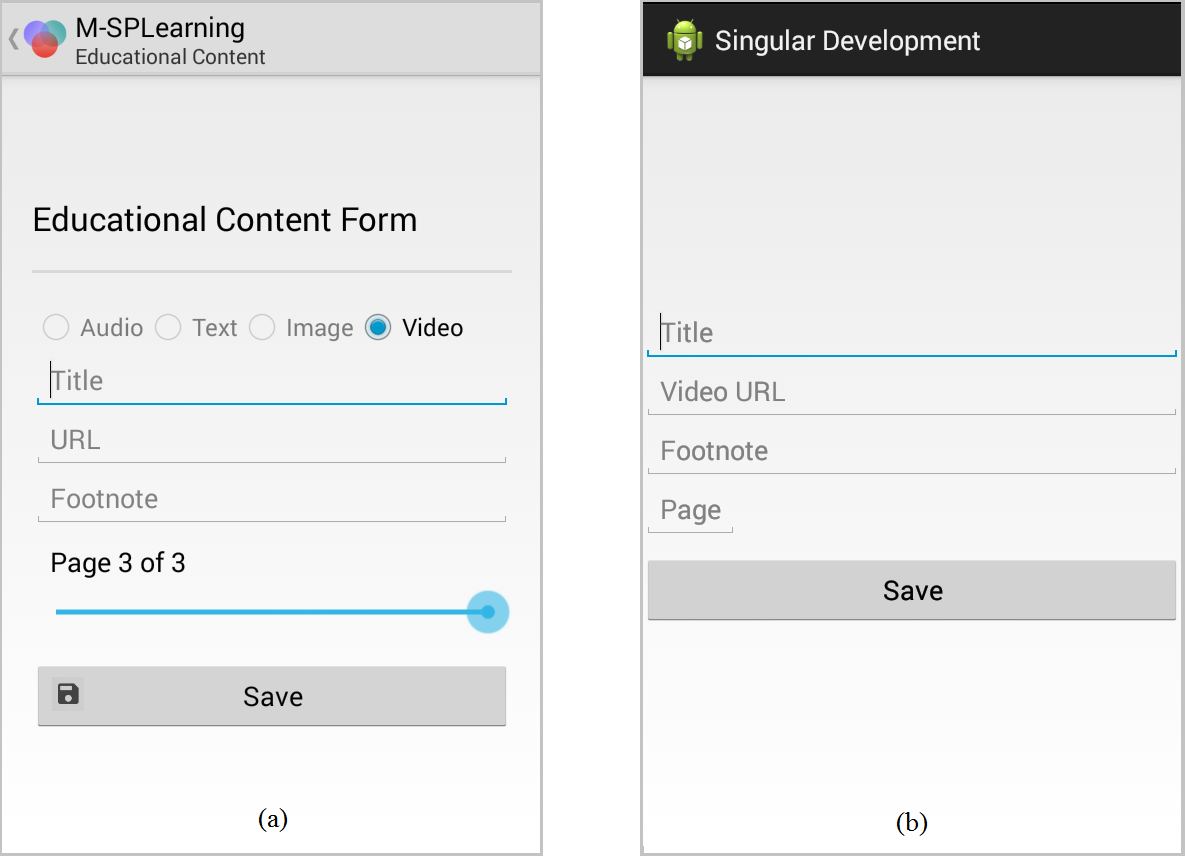
\includegraphics[scale=0.272]{figures/section4/prod.png}
\centering
\caption{Two Video Products (P1) Developed in the Experimental Execution with a) SPL and b) SDD.}
\label{fig:prod}
\end{figure*}


To collect the data for the analysis of time-to-market, the initial and final time of implementation process for P1 and P2, was registered individually in the experimental form to be calculated in Equation \ref{eq:1}. On the other hand, for the analysis of quality, each of 15 developed products were tested and the number of faults was collect to compare the use of SPL and SDD methodologies by means of the Equation \ref{eq:2}.

\subsubsection{Validity Evaluation}

A pilot project was developed with two pratictioners from industry, who evaluated the study instrumentation and established the duration of the training and execution sessions. The results and its participants were not used in the final execution and data analysis of the experiment.

\subsection{Execution}\label{sub:execution}

This section presents how the experimental plan (design) was defined.

\subsubsection{Sample}

The sample was composed of a total of 21 pratictioners who participated in the training session. However, 18 participants contributed in the experimental execution, due the unavailability of 3 volunteers in the execution day.

\subsubsection{Preparation}

The participants underwent a 3 day training of the essential concepts of Android development for SSD and SPL with the Eclipse IDE. The knowledge was evaluated through essays at the end of each training session. On the fourth day, the experiment was performed.

\subsubsection{Data Collection}

The steps adopted for data collection were:

\begin{enumerate}

\item the participants present of three daily 4 hour trainning sessions in an industrial environment;

\item the participants were divided into four groups by means of a draw;
\item the experimenter gave the participants a set of documents: containing UML diagram models, a dataset model and an interface message specification for each product, such as the material used in training session. Each individual was provided with a desktop computer with all requirements to develop a software product and received an experimental form to register the spending time with the development process for analysis.
\item the participant read each given document;
\item the experimenter explained the documents;
\item the participant read and clarified possible doubts about the products specifications; and
\item finally, each participant received and used two randomly drawn methodologies for the development of a requested m-learning product. For each application, participants registered the lasting of the application (start time, end and brakes). At the end of the two development tasks for the two methodologies they were asked to answer a feedback questionnaire and their opinion about the experimental execution and technologies used give.
\end{enumerate}

\subsection{Analysis}\label{sub:analysis}

As the experiment session was finished, collected data was prepared (tabulation and descriptive statistics) to be applied a statistical tests.

\subsubsection{Collected Data and Descriptive Statistics}

For each participant (``\texttt{Participant \#}'' column), we collected the following data: total time of implementation and total number of faults, identified by testing procedures, and the mean calculation. These results are shown in Table \ref{tab:resul1} and the results for each participant are plotted in box-plots of Figure \ref{fig:boxplot}. 

\begin{table}
\caption{\label{tab:resul1}SSD and SPL Collected Data and Descriptive Statistics.}
    \centering
    \scriptsize
\begin{tabular}{c|c|c|c|c}
\hline
\multirow{2}{*}{\textbf{Participant \#}} & \multicolumn{2}{c|}{\textbf{SSD}} & \multicolumn{2}{c}{\textbf{SPL}}  \\ \cline{2-5}
                                    & \textbf{Time $(t)$}   & \textbf{Faults $(f)$} & \textbf{Time $(t)$}  & \textbf{Faults $(f)$}                                  \\ \hline
1                                   & 161             & 15              & 2              & 9                                              \\ \hline
2                                   & 90              & 8               & 1              & 0                                             \\ \hline
3                                   & 105             & 4               & 11             & 0                                              \\ \hline
4                                   & 104             & 1               & 3              & 0                                             \\ \hline
5                                   & 73              & 2               & 1              & 0                                             \\ \hline
6                                   & 99              & 9               & 3              & 0                                              \\ \hline
7                                   & 165             & 12              & 10             & 0                                              \\ \hline
8                                   & 95              & 1               & 3              & 0                                              \\ \hline
9                                   & 104             & 3               & 2              & 0                                               \\ \hline
10                                  & 102             & 0               & 4              & 0                                              \\ \hline
11                                  & 61              & 0               & 2              & 0                                             \\ \hline
12                                  & 82              & 4               & 8              & 0                                              \\ \hline
13                                  & 114             & 1               & 4              & 0                                             \\ \hline
14                                  & 103             & 6               & 14             & 0                                            \\ \hline
15                                  & 111             & 2               & 2              & 0                                              \\ \hline
16                                  & 176             & 9               & 4              & 0                                              \\ \hline
17                                  & 120             & 17              & 5              & 0                                             \\ \hline
18                                  & 175             & 34              & 2              & 9                                              \\ \hline
\textbf{Mean}                       & \textbf{113.33} & \textbf{7.11}   & \textbf{4.50}  & \textbf{1.00}                 \\ \cline{1-5}
\textbf{Median}                     & \textbf{104}    & \textbf{4}      & \textbf{3}     & \textbf{0}                                      \\ \cline{1-5}
\textbf{Std. Dev.}                  & \textbf{33.98}  & \textbf{8.46}   & \textbf{3.75}  & \textbf{2.91}                             \\ \hline
\end{tabular}
\end{table}


\begin{figure}
\centering
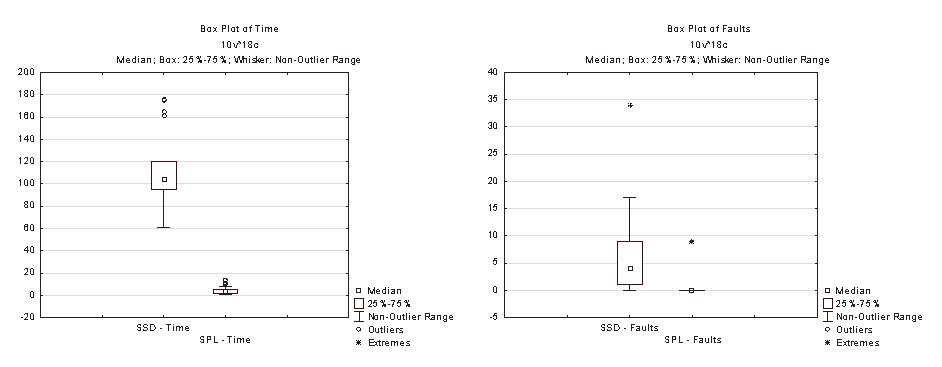
\includegraphics[scale=0.8]{./figures/section4/boxplot.eps}
\centering
\caption{Collected Data Box-Plot from SSD and SPL faults and SSD and SPL time-to-market.}
\label{fig:boxplot}
\end{figure}

\subsubsection{Hypothesis Testing}

Based on the results obtained by the use of SSD and SPL to the development of two mobile learning products, we summarize, analyze and interpret the SSD and SPL collected data (Table \ref{tab:resul1} and Figure \ref{fig:boxplot}) by means of the Shapiro-Wilk normality test and the Mann-Whitney-Wilcoxon hypothesis test. Both tests validated the statistical power of the sample, allowing test the hypothesis.

\subsubsection{Efficiency in the Time of Implementation (R.Q.1)}

\begin{itemize}

\item \textbf{Collected Data Normality Tests:} Shapiro-Wilk \cite{shaphirowilk65} normality test was applied to SSD and SPL time and faults and the following results were obtained:\\

\textbf{\textit{SSD time (\textit{N}=18):}}

For mean value ($\mu$) of 113.33 and standard deviation value of ($\sigma$) 33.98, the time for the SSD was \textit{p} = 0.0274.

In the \textit{Shapiro-Wilk} test for a sample size \textit{(N)} 18 with 95\% of significance level ($\alpha$ = 0.05), \textit{p} = 0.0274 (0.0274 $<$ 0.05) and calculated value of \textit{W} = 0.8813 $<$ \textit{W} = 0.8970, the sample is considered non-normal.

\textbf{\textit{SPL time (\textit{N}=18):}}

For mean value ($\mu$) of 4.50 and standard deviation value of ($\sigma$) 3.75, the time for the SPL was \textit{p} = 0.0014.

For a sample size \textit{(N)} 18 with 95\% of significance level ($\alpha$ = 0.05), \textit{p} = 0.0014 (0.0014 $<$ 0.05) and calculated value of \textit{W} = 0.7978 $<$ \textit{W} = 0.8970, the sample is considered non-normal.

\item \textbf{Mann-Whitney-Wilcoxon for SSD and SPL time samples:} a rank with weights was assigned to each sample value. The weights were added and applied in Equation \ref{eq:MWW}:
\small
\begin{equation}
\begin{split}
\label{eq:MWW}
U(DM) = N_1 * N_2 + \frac{N_1*(N_1+1)}{2} - \sum_{i=1}^{n} total_{2}
\end{split}
\end{equation}
\normalsize 
Where:
\begin{itemize}
\item \textit{$U(DM)$} is the equation for each independent sample (DM);
\item \textit{$N_1$} is the size of the sample for the X methodology;
\item \textit{$N_2$} is the size of the sample for the compared methodology (Y); and
\item \textit{$total_{2}$} is the sum of the weights given for the compared methodology.
\end{itemize}

The time values calculated by Equation \ref{eq:MWW} were 326.5 for SSD and 0.00 for SPL.

Each weight matches the participants weights of development process time with SSD or SPL methodology. There are evidences that both values are different ($326.5>0$), which leads to the rejection of the null hypothesis ($H_0$) and acceptance of the alternative hypothesis ($H_{2}$).

Therefore, the answer to R.Q.1 was: SPL is more efficient than the SSD to implement software products for mobile platform. The implementations of the base project and SPL were also considered in the experiment.

The participants received the base project of the two software products to be developed with SSD or SPL. It consists of similarities of the products and was developed to reduce the experimental execution duration. It was implemented in 480 minutes (8 hours).

If we consider the time required for the implementation of each project base, plus the total development time to each participants (480 minutes), the total time would be 10680 minutes or 178 hours ($total_{time}$((subje\allowbreak cts(18) x minutes(480)) + 2040 = 10680 minutes). Taking into account the base project, the time lasting by the 18 participants was 81 minutes (1 hour and 35 minutes) and the total time would be 11361 minutes or 189 hours and 35 minutes ($total_{time}$((participants(18) x minutes(4.5)) + 10599 = 11361 minutes). 

The comparison of the values, shows the SPL development spent 621 minutes (11 hours and 35 minutes) more than SSD. However, after the SPL implementation, this approach allows the evolution and insertion of new variabilities, guaranteeing the faster generation of new products in addition to other advantages of the adoption of SPL approach.

\end{itemize}

\subsubsection{Number of faults of the created software products (R.Q.2)}

\begin{itemize}

\item \textbf{Collected Data Normality Tests:} 

\textbf{\textit{SSD faults (\textit{N}=18):}}

For a mean value ($\mu$) 7.11 and standard deviation value of ($\sigma$) 4, the fault for the SSD was \textit{p} = 0.0006 for the \textit{Shapiro-Wilk} normality test.

For a sample size \textit{(N)} 18 with 95\% significance level ($\alpha$ = 0.05), \textit{p} = 0.0006 (0.0006 $<$ 0.05) and value of \textit{W} = 0.7740 $<$ \textit{W} = 0.8970, the sample is considered non-normal.

\textbf{\textit{SPL faults (\textit{N}=18):}}

For a mean value ($\mu$) 1.00 and standard deviation value of ($\sigma$) 0, the fault for the SPL was \textit{p} = 0.00000007 for the \textit{Shapiro-Wilk} normality test.

For a sample size \textit{(N)} 18 with 95\% of significance level ($\alpha$ = 0.05), \textit{p} = 0.00000007 (0.00000007 $<$ 0.05) and value of \textit{W} = 0.3730 $<$ \textit{W} = 0.8970, the sample is considered non-normal.

\item \textbf{Mann-Whitney-Wilcoxon for SSD and SPL faults samples:} the number of faults calculated for SSD by Equation \ref{eq:MWW} was 282, whereas and for SPL, it was 42.

Each weight matches participants development project faults with SSD or SPL methodology. There are evidences that both values are different ($282>42$), which leads to the rejection of the null hypothesis ($H_0$) and acceptance of the alternative hypothesis ($H_{1}$).

According to the result from the Mann-Whitney-Wilcoxon, the answer for R.Q.2 was obtained: it means that the SSD is prone to showed more faults in the software products developed than the SPL.

\end{itemize}

\subsection{Interpretation and Discussion}\label{sub:interpretation}

Data collected from the SSD and SPL application was analyzed and interpreted. The results are summarized in Table \ref{tab:resul_s}.

\begin{table}
\caption{\label{tab:resul_s}SSD and SPL Normality and Statistical Tests Results.}
\centering
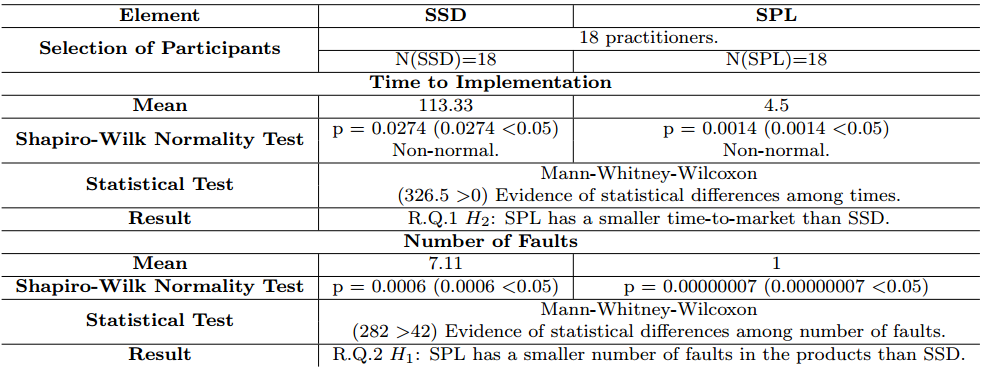
\includegraphics[scale=0.35]{figures/section4/MSPLExpSummary.png}

%\scriptsize
%\resizebox{0.87\textwidth}{!}{\begin{minipage}{\textwidth}
%\begin{tabular}{ccc}
%\hline
%\multicolumn{1}{c|}{\textbf{Element}}                                      & \multicolumn{1}{c|}{\textbf{SSD}}                          & \textbf{SPL}                                 \\ \hline
%\multicolumn{1}{c|}{\multirow{2}{*}{\textbf{Selection of Participants}}}       & \multicolumn{2}{c}{18 practitioners.}                                                                     \\ \cline{2-3} 
%\multicolumn{1}{c|}{}                                                      & \multicolumn{1}{c|}{N(SSD)=18}                             & N(SPL)=18                                    \\ \hline
%\multicolumn{3}{c}{\textbf{Time to Implementation}}                                                                                                                                            \\ \hline
%\multicolumn{1}{c|}{\textbf{Mean}}                                         & \multicolumn{1}{c|}{113.33}                                & 4.5                                          \\ \hline 
%\multicolumn{1}{c|}{\multirow{2}{*}{\textbf{Shapiro-Wilk Normality Test}}} & \multicolumn{1}{c|}{p = 0.0274 (0.0274 \textless 0.05)}    & p = 0.0014 (0.0014 \textless 0.05)           \\
%\multicolumn{1}{c|}{}                                                      & \multicolumn{1}{c|}{Non-normal.}                           & Non-normal.                                  \\ \hline
%\multicolumn{1}{c|}{\multirow{2}{*}{\textbf{Statistical Test}}}            & \multicolumn{2}{c}{Mann-Whitney-Wilcoxon}                                                                 \\
%\multicolumn{1}{c|}{}                                                      & \multicolumn{2}{c}{(326.5 \textgreater 0) Evidence of statistical differences among times.}            \\ \hline
%\multicolumn{1}{c|}{\textbf{Result}}                                       & \multicolumn{2}{c}{R.Q.1 $H_2$: SPL has a smaller time-to-market than SSD.}                                                      \\ \hline
%\multicolumn{3}{c}{\textbf{Number of Faults}}                                                                                                                                \\ \hline
%\multicolumn{1}{c|}{\textbf{Mean}}                                         & \multicolumn{1}{c|}{7.11}                                  & 1                                            \\ \hline
%\multicolumn{1}{c|}{\textbf{Shapiro-Wilk Normality Test}}                  & \multicolumn{1}{c|}{p = 0.0006 (0.0006 \textless 0.05)}    & p = 0.00000007 (0.00000007 \textless 0.05)   \\ \hline
%\multicolumn{1}{c|}{\multirow{2}{*}{\textbf{Statistical Test}}}            & \multicolumn{2}{c}{Mann-Whitney-Wilcoxon}                                                                 \\
%\multicolumn{1}{c|}{}                                                      & \multicolumn{2}{c}{(282 \textgreater 42) Evidence of statistical differences among number of faults.} \\ \hline
%\multicolumn{1}{c|}{\textbf{Result}}                                       & \multicolumn{2}{c}{R.Q.2 $H_1$: SPL has a smaller number of faults in the products than SSD.}                                    
%\end{tabular}
%\end{minipage}}
\end{table}

In terms of time-to-market, the statistical difference showed by Mann-Whitney-Wilcoxon test provides evidence that SPL (i.e., M-SPLear\allowbreak ning) was more efficient than SSD in the development of P1 and P2 m-learning products, therefore, R.Q.1 has been answered.

Regarding number of faults, the statistical difference presented by Mann-Whitney-Wilcoxon test provides evidence that SSD showed more faults than SPL in the development of P1 and P2 m-learning products, therefore, R.Q.2 has been answered.

According to the results of the Mann-Whitney-Wilcoxon test, both R.Q.1 and R.Q.2 null hypotheses can be rejected.

\subsubsection{Threats to Validity}\label{sec:threats}

This section addresses the actions taken to play directly against threats of this experiment, according to the Conceptual Model of Anderlin Neto and Conte \cite{neto13}.

\textbf{Internal Validity:}

\begin{itemize}
\item \textbf{Differences among participants:} as we selected participants with different experience levels, variations in this skills were reduced during the training sessions. The assessments conducted at in the end of each day of training demonstrated the level of knowledge in the content used in the experimental execution and guaranteed the reduction in variations in the participants skills. Even knowing that a more homogeneous sample reduce the subjects representativeness, it was decided to apply the training to reduce the heterogeneity of participants, that could threat the conclusion validity.

\item \textbf{Fatigue effects:} on average, the experiment lasted 180 minutes. Fatigue was not considered relevant since the participants could leave the room for a quick break. They were warned to not communicate during the breaks and, to guarantee, an human observer supervised them. Periods of absence were registered and disregarded in the time analysed.



\item \textbf{Influence among participants:} the participants performed the experiment under the supervision of a human observer, so that a possible influence of communication among them could be mitigated. As participants behaves differently when being observed, training sessions allowed the adaptation the participants to the environment, reducing this threat.

\item \textbf{Trainning Sessions:} in the training sessions, explanations were given for every participant. This action was taken to avoid possible biases, and allow that every training member solve all your questions.
\end{itemize}

\textbf{External Validity:}

\begin{itemize}

\item \textbf{Instrumentation:} m-learning products and other instruments were tested in the pilot project and were considered significant for the analysis of time-to-market and number of faults.

\item \textbf{Participants:} more experiments that considering different metrics with industry practitioners must be conducted for the identification of other relevant factors related to the adoption of M-SPLear\allowbreak ning.

\end{itemize}

\begin{itemize}

\item \textbf{Construction Validity:} independent variables were tested in the pilot project to guarantee their validity.

\item \textbf{Conclusion Validity:} since the number of participants is reduced, mainly by the availability of practitioners in the industry, the sample size must be increased in prospective replications of the experiment. Our results are considered indicators and are not conclusive, although the lack of experimental executions in an industrial environment, even with small samples, is important for the evaluation of the time-to-market and quality for both SSD and SPL.

\end{itemize}


\section{Lessons Learned}\label{section5}

During the execution of the activities documented in this paper, the authors identified some situations in which works related to the concepts involved can benefit. As lessons learned we highlight:

\begin{itemize}
    \item \textbf{Domain Characteristics:} a domain analysis can be considered one of the most important activities for the creation of an SPL. The evolution of the catalog of requirements proposed by Duarte Filho and Barbosa \cite{filho13} significantly contributed in terms of domain knowledge and supported the adoption of the proactive model for the development of M-SPLear\allowbreak ning.
    \item \textbf{Variability Management:} the use of the SMarty notation helps the identification of the variation points during the design of M-SPLear\allowbreak ning, ensuring greater cohesion for the implementation of the SPL components. It also contributes to the assimilation of the SPL concept. However, those involved must be trained so that the elements of notation can be used consistently.
    \item \textbf{SPL Architecture:} SPL needs mechanisms to allow a transparent and easy manner to reflect all updates in the core assets in the architecture, and vice versa, in other words, changes to the core assets require more efforts to maintain architectural integrity. Additional tools and analysis must be done to guarantee that all changes, in the architecture or in the components is reflecting all features and behaviors that the line have until that moment.
    \item \textbf{SPL Development:} considering the M-SPLear\allowbreak ning, the implementation of something generic and customizable is significantly different from a static approach. Therefore, developing features in an SPL requires a greater effort, which is justified by the subsequent gains of reuse.

On another hand, the singular development methodology makes it difficult the maintenance of the products, without any rigorous development process defined. As all developers tend to program in their own way, give support for each product developed, in most cases, could take most time and cost more. If an SPL practice is adopted, and is rigorously followed, the cost and time to give support tend to decrease.
    \item \textbf{Experimental Evaluation:} researches show that test executions in SPL are scarce and need to be evaluated and validated \cite{engstrom11}. Thus, the authors decided to apply the test cases in the products generated by the SPL, enabling a interesting comparison with an alternative methodology of development.
  
The experimental evaluation provided relevant results for the adoption of M-SPLear\allowbreak ning. The choice for active participants in the industry contributed to the reduction of the training session. However, experience and understanding the concepts by the participants is always difficult to measure.
\end{itemize}

Moreover, the use of tests techniques in the traditional development process and new ways to test quickly products from an SPL require more attention and research. One benefit in the adoption of SPL is about the improve of quality, since the products and their components are testing in several instantiations, leading to a quickly fix for the final client. Although the use of the components in a large number of products and, for consequently, a bigger number of target users for SPL, the way that the components and products were tested could be improved to be done in more aligned way with the SPL specificities. Literature reflects more concern to test the SPL architecture and fewer preoccupation to test the final components and products.

\section{Related Work} \label{section6}

%There is a lack on literature with regard to the use of variabilities and SPL to create mobile learning applications, as it is possible to note by searching terms as ``mobile learning software product line'', ``mobile learning variabiliti'' and variations, in ACM\footnote{http://dl.acm.org/} or IEEE\footnote{http://ieeexplore.ieee.org/} search bases. Therefore, the related works has a different focus of mobile learning, although, they specify and present some open issues to be researched and explored.

Gamez et al. \cite{gamez14} proposed a self-adaptation of mobile systems with dynamic SPLs. The management of variabilities is achieved using the Common Variability Language (CVL). The authors claim that CVL allows modeling the variability separately from the base model, but both the variability and the base models appear as connected and can be managed using the same tool. %The proposal was applied in a case study and presents good results.

Marinho et al. \cite{marinho10} proposed an architecture for nested SPLs in the domain of mobile and context-aware applications. However, the authors did not specify how to improve the management of variabilities. %The strategy used was defined a nested SPL that aims to facilitate the construction of such software by domain decompostition in two level of analysis. 

Bezerra et al. \cite{bezerra09} conducted a systematic review of SPLs applied to mobile middlewares, but only six studies were significant for the review. According to the authors, the few results obtained highlight the need of more research in the area. %In the specification of techniques used to developed SPLs in to mobile middleware, standed out feature model and domain specific language.

In another systematic literature review, Chen and Babar \cite{chen11} concluded the status of evaluation of variability management approaches in SPL engineering was quite dissatisfactory.

Actually, there are several opportunities and open issues regarding the management of variabilities and experimental evaluation, particularly in the m-learning domain. Such needs of research in the area has motivated our work.

%It is clearly visible that the related works is not directly related with our study. This few works motivated the research to analise the variabilities in the mobile learning context. The paucity of researchs presents the necessity to investigate the mainly issues and opened oportunities to explore them, such as the application of them in educational context. Other visible lack in the literature is related the experimental validation to compare the time-to-market and quality of products developed with SPL and SSD methodologies, as metioned by Chen and Muhammad \cite{chen2011systematic}.

%As can be seen, there is a need for investigating variability management in several context, research  to investigate the mainly issues and opened oportunities to explore them, such as the application of them in educational context lack of As pointed out by Chen and Muhammad \cite{chen2011systematic}. Other visible lack in the literature is related the experimental validation to compare the time-to-market and quality of products developed with SPL and SSD methodologies, as metioned by Chen and Muhammad \cite{chen2011systematic}.

%The needs to explore them and experimentally evaluation the real beneficts of this methodology it is justify, not only by the reports in software product line studies in other domains, but the possibilite of the adoption of a variability management approach and SPL paradigm as a new oportunity to replace the traditional single development.

%A incipiência de estudos experimentais no contexto de linhas de produto, que comparem este paradigma de reutilização de artefatos de software com outras metodologias de desenvolvimento é claramente visível, como menciona Chen e Muhamad em sua revisão sistemática da literatura \cite{chen2011systematic}. A escassez de trabalhos neste sentido levou a busca de trabalhos isolados de avaliação de paradigmas de desenvolvimento para a condução do presente estudo. 


\section{Conclusions and Future Work}\label{section7}

%Atualmente, de acordo com a International Telecommunication Union (ITU), a quantidade de assinaturas móveis em todo o mundo aproxima-se do número de pessoas na terra. Nesse contexto, a plataforma Android mostrou-se mais relevante no domínio das aplicações m-learning, devido a sua quantidade de usuários potenciais. Com isso, este trabalho propõe uma LPS cujo principal objetivo é proporcionar maior reúso e padronização para esse domínio de aplicações.
%Nowadays, according to the International Telecommunication Union (ITU) \cite{itu14}, the number of mobile subscriptions around the world approaches the number of people on Earth. In this context, the Android platform was more relevant in the field of m-learning applications, due to its amount of potential users. Thus, 
This work proposes an SPL main objective is to provide greater reuse and standardization for producing m-learning applications.
%For this, we discussed how the variability management can improve the development of software products, particularly in the context of m-learning applications. We described M-SPLear\allowbreak ning, which supports the development of customizable m-learning applications according to the basics of SPLs.
%Nesse cenário, o tempo necessário para o desenvolvimento dessas aplicações é essencial para que elas cheguem mais rapidamente a seus usuários finais. Desta forma, o estudo do conceito de LPS convergiu com a necessidade em questão e resultou na concepção da M-SPLear\allowbreak ning.
In this scenario, the time required for the development of such applications is essential to come more quickly to their end users. Thus, the study of the concept of SPL converged to the need in question and resulted in the conception of M-SPLear\allowbreak ning.

To support our ideas, we experimentally evaluated the use of M-SPLear\allowbreak ning with respect to the singular software development. The obtained results were significant for the reuse approach, showing a reduction on time-to-market and a better quality in terms of faults when considering the software products developed with the support of variabilities. 

It is also important to highlight that the SMarty approach was crucial to the development of M-SPLear\allowbreak ning, providing cost savings and better quality to the software products developed.

%Como trabalhos futuros, pretende-se evoluir a M-SPLear\allowbreak ning com base nos insumos fornecidos a partir de sua avaliação empírica. Nesse sentido, ainda existe uma quantidade significativa de informações que podem induzir a novas linhas de pesquisa e avaliações experimentais.
As future work, we intend to evolve M-SPLear\allowbreak ning based on the inputs provided by the empirical evaluation performed. In this sense, there is still a significant amount of information that can lead to new research lines and experimental evaluations.

%Além disso, para que a M-SPLear\allowbreak ning possa ser avaliada em sua totalidade, todas as features elicitadas pelo catálogo de requisitos devem ser devidamente implementadas. Desta forma, um estudo empírico envolvendo a LPS propriamente dita pode ser conduzido, porque nosso experimento aferiu apenas os produtos da M-SPLear\allowbreak ning.
Moreover, to a whole evaluation of M-SPLear\allowbreak ning, all features elicited by catalog requirements must be properly implemented. Therefore, an empirical study involving the LPS itself can be conducted, because our experiment measured only M-SPLear\allowbreak ning products.

%Considerando o domínio explorado, a plataforma Android vem recebendo constantes contribuições em sua estratégia de desenvolvimento. Com isso, o aperfeiçoamento da M-SPLear\allowbreak ning deve sempre considerar a avaliação de novas ferramentas, fazendo com que a LPS evolua de acordo com as tendências do mercado.
%Considering the explored domain, the Android platform has received ongoing contributions to its development strategy. Thus, the improvement of M-SPLear\allowbreak ning must always consider the evaluation of new tools, causing the LPS evolve according to market trends.

%Para avaliação das evoluções da M-SPLear\allowbreak ning novos experimentos devem ser conduzidos, explorando vertentes relevantes para contexto educacional. Nesse sentido, avaliar os produtos gerados considerando variáveis como usabilidade e efetividade devem proporcionar resultados expressivos para este estudo. Além disso, as aplicações móveis resultantes podem ser aplicadas  em cenários reais de ensino e aprendizagem, com o objetivo de avaliar a M-SPLear\allowbreak ning aplicada ao seu domínio de usuários.
%evolutions of 
To evaluate the M-SPLear\allowbreak ning new experiments should be conducted, exploring relevant  aspects to educational context. In this sense, evaluate the products considering variables such as usability and effectiveness should provide significant results for this study. In addition, the resulting mobile applications can be applied in real scenarios of teaching and learning, in order to evaluate the M-SPLear\allowbreak ning applied to your potential users.

%Outra perspectiva interessante está relacionada à investigação das outras estratégias de adoção propostas por. O modelo extrativo poderia ser aplicado a produtos externos a M-SPLear\allowbreak ning, com o objetivo de expandir suas features. Além disso, o modelo reativo poderia ser estudado como uma alternativa para evoluções futuras da LPS proposta.
We also intend to investigate the use of other adoption models \cite{krueger02}. For instance, the extractive model can be applied in similar products to those generated by M-SPLear\allowbreak ning aiming at increasing the validity of similarities and variabilities specified. The reactive model can be investigated as an alternative to the evolution of the proposed SPL as well.

\begin{acknowledgements}
We would like to thank the Brazilian funding agencies (FAPESP 2014/03389-9, CAPES, CNPq) for their support.
\end{acknowledgements}

\begin{thebibliography}{99}

\harvarditem{Chen}{2011}{chen11} Chen~L, Babar~MA. 2011. A systematic review of evaluation of variability management approaches in software product lines. Information and Software Technology.

\harvarditem{Capilla et al}{2013}{capilla13} Capilla~R, Bosch~J, Kang~KC. 2013. Systems and Software Variability Management. Springer.

\harvarditem{B\"{o}ckle and van der Linden}{2005}{bockle05} B\"{o}ckle~G, van der Linden~FJ. 2005. Software product line engineering: foundations, principles and techniques. Edited by Klaus Pohl. Springer Science \& Business Media.

\harvarditem{van der Linden et al}{2007}{vanderlinden07} van der Linden~FJ, Schmid~K, Rommes~E. 2007. Software product lines in action: the best industrial practice in product line engineering. Springer Science \& Business Media.

\harvarditem{West and Vosloo}{2012}{west12} West~M, Vosloo~S. 2012. Mobile Learning for Teachers: Global Themes. UNESCO.

\harvarditem{Kukulska-Hulme and Traxler}{2005}{kukulska05} Kukulska-Hulme~A, Traxler~J. 2005. Mobile Learning: a Handbook for Educators and Trainers. Routledge.

\harvarditem{Bezerra et al}{2009}{bezerra09} Bezerra~YM, Pereira~TAB, da Silveira~GE. 2009. A Systematic Review of Software Product Lines Applied to Mobile Middleware. Information Technology: New Generations (ITNG).

\harvarditem{Kinshuk et al}{2003}{kinshuk03} Kinshuk~SJ, Sutinen~E, Goh~T. 2003. Mobile technologies in support of distance learning. Asian Journal of Distance Education.

\harvarditem{Wexler et al}{2008}{wexler08} Wexler~S, Brown~J, Metcalf~D, Rogers~D, Wagner~E. 2008. Mobile Learning: What it is, why it matters, and how to incorporate it into your learning strategy. Guild Research.

\harvarditem{FalvoJr et al}{2014a}{falvojr14a} FalvoJr~V, Duarte Filho~NF, OliveiraJr~E, Barbosa~EF. 2014. Towards the Establishment of a Software Product Line for Mobile Learning Applications. International Conference on Software Engineering and Knowledge Engineering (SEKE).

\harvarditem{FalvoJr et al}{2014b}{falvojr14b} FalvoJr~V, Duarte Filho~NF, OliveiraJr~E, Barbosa~EF. 2014. A Contribution to the Adoption of Software Product Lines in the Development of Mobile Learning Applications. Annual Frontiers In Education (FIE) Conference.

\harvarditem{OliveiraJr et al}{2010}{oliveirajr10} OliveiraJr E, Gimenes IMS, Maldonado JC. 2010. Systematic Management of Variability in UML-based Software Product Lines. Journal Universal Computer Science.

\harvarditem{Bosch}{2001}{bosch01} Bosch~J. 2001. Software product lines: organizational alternatives. International Conference on Software Engineering.

\harvarditem{Marcolino et al}{2013}{marcolino13} Marcolino~A, OliveiraJr~E, Gimenes~IMS, Maldonado~JC. 2013. Towards the Effectiveness of a Variability Management Approach at Use Case Level. International Conference on Software Engineering and Knowledge Engineering (SEKE).

\harvarditem{Marcolino et al}{2014a}{marcolino14a} Marcolino~A., OliveiraJr~E, Gimenes~IMS, Barbosa~EF. 2014. Empirically Based Evolution of a Variability Management Approach at UML Class Level. Computer Software and Applications Conference (COMPSAC).

\harvarditem{Marcolino et al}{2014b}{marcolino14b} Marcolino~A., OliveiraJr~E, Gimenes~IMS. 2014. Towards the Effectiveness of the SMarty Approach for Variability Management at Sequence Diagram Level. International Conference on Enterprise Information Systems (ICEIS).

\harvarditem{Bera et al}{2015}{bera15} Bera~MHG, OliveiraJr~E, Colanzi~TE. 2015. Evidence-based SMarty Support for Variability Identification and Representation in Component Models. International Conference on Enterprise Information Systems (ICEIS).

\harvarditem{Duarte~Filho and Barbosa}{2013}{filho13} Duarte~Filho~NF, Barbosa~EF. 2013. A requirements catalog for mobile learning environments. Annual ACM Symposium on Applied Computing.

\harvarditem{Krueger}{2002}{krueger02} Krueger~C. 2002. Easing the transition to software mass customization. Software Product-Family Engineering. Springer Berlin Heidelberg.

\harvarditem{Kang et al}{1990}{kang90} Kang~KC, Cohen~SG, Hess~JA, Novak~WE, Peterson~AS. 1990. Feature-oriented domain analysis (FODA) feasibility study. Software Engineering Institute, Carnegie Mellon University.

\harvarditem{Llamas et al}{2014}{llamas14} Llamas~MSR, Reith~R, Shirer~M. 2014. Android and iOS Continue to Dominate the Worldwide Smartphone Market with Android Shipments Just Shy of 800 Million in 2013. According to IDC (Online).

\harvarditem{Van Gurp et al}{2001}{vangurp01} Van Gurp~J, Bosch~J, Svahnberg~M. 2001. On the notion of variability in software product lines. Working IEEE/IFIP Conference on Software Architecture.

\harvarditem{Fielding}{2000}{fielding00} Fielding~RT. 2000. Architectural styles and the design of network-based software architectures. University of California.

\harvarditem{Marinho et al}{2010}{marinho10} Marinho~FG, Costa~AL, Lima~FF, Neto~JBB, Rocha~L, Dantas~VLL, Andrade~RMC, Teixeira~E, Werner~C. 2010. An architecture proposal for nested software product lines in the domain of mobile and context-aware applications. Software Components, Architectures and Reuse (SBCARS).

\harvarditem{Nascimento et al}{2011}{nascimento11} Nascimento~AS, Rubira~CMF and Lee~J. 2011. An SPL approach for adaptive fault tolerance in SOA. International Software Product Line Conference.

\harvarditem{Jedlitschka and Pfahl}{2005}{jedlitschka07} Jedlitschka~A, Pfahl~D 2005. Reporting guidelines for controlled experiments in software engineering. In Empirical Software Engineering. IEEE Software.

\harvarditem{Wohlin et al}{2012}{wohlin12} Wohlin~C, Runeson~P, Host~M, Ohlsson~MC, Regnell~B, Wesslen~A. 2012. Experimentation in software engineering. Springer Science \& Business Media.

\harvarditem{Juristo and Moreno}{2010}{juristo10} Juristo~N and Moreno~ AM. 2010. Basics of Software Engineering Experimentation (1st ed.). Springer Publishing Company, Incorporated.

\harvarditem{Craig and Jaskiel}{2002}{craig02} Craig~RD, Jaskiel~SP. 2002. Systematic software testing. Artech House.

\harvarditem{Shaphiro and Wilk}{1965}{shaphirowilk65} Shaphiro~SS, Wilk~MB. 1965. An analysis of variance test for normality. Biometrika.

\harvarditem{Neto and Conte}{2013}{neto13} Neto~AA, Conte~T. 2013. A conceptual model to address threats to validity in controlled experiments. International Conference on Evaluation and Assessment in Software Engineering. ACM.

\harvarditem{Engstr\"{o}m and Runeson}{2011}{engstrom11} Engstr\"{o}m~E, Runeson~P. 2011. Software product line testing -- A systematic mapping study. Information and Software Technology.

\harvarditem{Gamez et al}{2014}{gamez14} Gamez~N, Fuentes~L, Troya~J. 2014. Self-adaptation of mobile systems with dynamic software product lines. IEEE Software.

\harvarditem{ITU}{2014}{itu14} ITU. 2014. The world in 2014: Ict facts and figures. Information and Communication Technologies (ICT).

\harvarditem{Jaring and Bosch}{2002}{jaring02} Jaring M and Bosch J. 2002. "Representing Variability in Software Product Lines: A Case Study," in Software Product Lines : Second International Conference, SPLC 2, San Diego, CA, USA, August 19-22, 2002. Proceedings, vol. LNCS 2379, G. Chastek, Ed.: Springer Berlin / Heidelberg, pp. 219-245.

\harvarditem{Hubaux et al}{2010}{hubaux10} Hubaux A, Boucher Q, Hartmann H, Michel R, and Heymans P. 2010. "Evaluating a Textual Feature Modelling Language: Four Industrial Case Studies," presented at 3rd International Conference on Software Language Engineering (SLE'10), Eindhoven, Netherlands.

\harvarditem{Eriksson et al}{2009}{eriksson09} Eriksson M, Börstler J, and Kjell B. 2009. "Managing requirements specifications for product lines - An approach and industry case study," Journal of Systems and Software, vol. 82, pp. 435-447.

\harvarditem{Ardis et al}{2000}{ardis00} Ardis M, Daley N, Hoffman D, Siy H, and Weiss D. 2000. "Software product lines: a case study," Software: Practice and Experience, vol. 30, pp. 825-847.

\harvarditem{Gacek et al}{2001}{gacek01} Gacek C, Knauber P, Schmid K, and Clements P. 2001. "Successful Software Product Line Development in a Small Organization - A Case Study," IESE-Report No. 013.01/E, Fraunhofer IESE.

\harvarditem{Batory et al}{2002}{batory02} Batory D, Johnson C, MacDonald B, and von Heeder D. 2002. "Achieving Extensibility Through Product-Lines and Domain-Specific Languages: A Case Study," ACM Transactions on Software Engineering and Methodology, vol. 11, pp. 191-214.

\end{thebibliography}

\section*{Author Biographies}
\leavevmode

\vbox{%
\begin{wrapfigure}{l}{80pt}
{\vspace*{15pt}\fbox{insert photo}\vspace*{100pt}}%
\end{wrapfigure}
\noindent\small 
{\bf Venilton FalvoJr} TODO \vadjust{\vspace{40pt}}}

\vspace{15pt}
\vbox{%
\begin{wrapfigure}{l}{80pt}
{\vspace*{15pt}\fbox{insert photo}\vspace*{100pt}}%
\end{wrapfigure}
\noindent\small {\bf Anderson~Marcolino} TODO \vadjust{\vspace{40pt}}}

\vspace{15pt}
\vbox{%
\begin{wrapfigure}{l}{80pt}
{\vspace*{15pt}\fbox{insert photo}\vspace*{100pt}}%
\end{wrapfigure}
\noindent\small 
{\bf Nemesio~Duarte~Filho} TODO \vadjust{\vspace{40pt}}}

\vspace{15pt}
\vbox{%
\begin{wrapfigure}{l}{80pt}
{\vspace*{15pt}\fbox{insert photo}\vspace*{100pt}}%
\end{wrapfigure}
\noindent\small 
{\bf Edson~OliveiraJr} TODO \vadjust{\vspace{40pt}}}

\vspace{15pt}
\vbox{%
\begin{wrapfigure}{l}{80pt}
{\vspace*{15pt}\fbox{insert photo}\vspace*{100pt}}%
\end{wrapfigure}
\noindent\small 
{\bf Ellen~Barbosa} TODO \vadjust{\vspace{40pt}}}

\correspond{Ellen Barbosa, Institute of Science and Computational Mathematics (ICMC-USP), Avenida Trabalhador S\~ao-Carlense, 400, S\~ao Paulo, Brazil. E-mail: francine@icmc.usp.br. Phone: +55 (16) 3373-8177. Fax: +55 (16) 3373-8888.}
\label{lastpage}
\end{document}
